
%%%%%%%%%%%%%%%%%%%%%%%%%%%%%%%%%%%%%%%%%
% Thesis LaTeX Template
%
% This template has been downloaded from:
% http://www.latextemplates.com
%
% Original authors:
% Steven Gunn 
% http://users.ecs.soton.ac.uk/srg/softwaretools/document/templates/
% and
% Sunil Patel
% http://www.sunilpatel.co.uk/thesis-template/
%
% Note:
% Make sure to edit document variables in the Thesis.cls file
%
%%%%%%%%%%%%%%%%%%%%%%%%%%%%%%%%%%%%%%%%%

%----------------------------------------------------------------------------------------
%	PACKAGES AND OTHER DOCUMENT CONFIGURATIONS
%----------------------------------------------------------------------------------------

\documentclass[11pt, a4paper, oneside]{Thesis} % Paper size, default font size and one-sided paper

\graphicspath{{./Pictures/}} % Specifies the directory where pictures are stored
\newcommand{\BigO}[1]{\ensuremath{\operatorname{O}\bigl(#1\bigr)}}
\usepackage{algorithm}% http://ctan.org/pkg/algorithm
\usepackage{algpseudocode}% http://ctan.org/pkg/algorithmicx
\usepackage{arabtex,utf8}
\usepackage{color}
\definecolor{dkgreen}{rgb}{0,0.6,0}
\definecolor{gray}{rgb}{0.5,0.5,0.5}
\definecolor{mauve}{rgb}{0.58,0,0.82}
\usepackage[square, numbers, comma, sort&compress]{natbib} % Use the natbib reference package - read up on this to edit the reference style; if you want text (e.g. Smith et al., 2012) for the in-text references (instead of numbers), remove 'numbers' 
\hypersetup{urlcolor=blue, colorlinks=true} % Colors hyperlinks in blue - change to black if annoying
\title{\ttitle} % Defines the thesis title - don't touch this

\begin{document}
\setcode{utf8}
\frontmatter % Use roman page numbering style (i, ii, iii, iv...) for the pre-content pages

\setstretch{1.3} % Line spacing of 1.3

% Define the page headers using the FancyHdr package and set up for one-sided printing
\fancyhead{} % Clears all page headers and footers
\rhead{\thepage} % Sets the right side header to show the page number
\lhead{} % Clears the left side page header

\pagestyle{fancy} % Finally, use the "fancy" page style to implement the FancyHdr headers

\newcommand{\HRule}{\rule{\linewidth}{0.5mm}} % New command to make the lines in the title page

%----------------------------------------------------------------------------------------
%	TITLE PAGE
%----------------------------------------------------------------------------------------

\begin{titlepage}
\begin{center}

\textsc{\LARGE Alexandria University}\\[1.5cm] % University name
\textsc{\Large Graduation Project}\\[0.5cm] % Thesis type

\HRule \\[0.4cm] % Horizontal line
{\huge \bfseries Semantic based Arabic-news Clustering and Recommendation}\\[0.4cm] % Thesis title
%{\huge \bfseries Applied to News Reommender System}\\[0.4cm] % Thesis title
\HRule \\[1cm] % Horizontal line

\large \textit{Supervisor:}\\[0.4cm]
\begin{minipage}{0.4\textwidth}
\begin{center} \large
Prof. Dr. Nagwa M. El-Makky\\
Dr. Noha A. Yousri 
% Supervisor name - remove the \href bracket to remove the link  
\end{center}
\end{minipage}\\[1cm]
 
\large \textit{Members:}\\[0.4cm]
\begin{minipage}{0.4\textwidth}
\begin{center} \large
Ahmed Hesham Emara \\  Ahmed Mahmoud El-bagoury \\ 
Ahmed Mohamed Mohsen \\ Samer Samy Meggaly \\
Mohamed Gaber El-sayed
\end{center}
\end{minipage}\\[1cm]
 
\large \textit{A thesis submitted in fulfilment of the requirements\\ for the degree of Bachelor }\\[0.4cm] % University requirement text
Computer \& System Engineering Department\\[0.7cm] % Research group name and department name
 
{\large \today}\\[0.4cm] % Date

\includegraphics{./Figures/Logo_Alexandria_University.png} % University/department logo - uncomment to place it
\vfill 
\end{center}

\end{titlepage}


%----------------------------------------------------------------------------------------
%	ABSTRACT PAGE
%----------------------------------------------------------------------------------------

\addtotoc{Abstract} % Add the "Abstract" page entry to the Contents

\abstract{\addtocontents{toc}{\vspace{1em}} % Add a gap in the Contents, for aesthetics
The dramatic change of the political scene in the Middle East especially in the Arabic nations has resulted in significant increase in the flow of the Arabic news through the web and social networks, accompanied with readers passion to keep track with all news.Also presence of many online-news sources that possess different point of views, many stories may exist for the same piece of news.\newline
Here arouses the need for an automated system that groups the similar news from different sources to ease browsing and enables the user to follow up the whole story from different perspectives. We managed to build a semantic based system to tackle these problems, as lexical techniques may result in ambiguity as Arabic language contains many synonyms for the same word and it is highly derivative  language where tens or even hundreds of words could be
formed using only one root.
}

\clearpage % Start a new page

%----------------------------------------------------------------------------------------
%	ACKNOWLEDGEMENTS
%----------------------------------------------------------------------------------------

\setstretch{1.3} % Reset the line-spacing to 1.3 for body text (if it has changed)

\acknowledgements{\addtocontents{toc}{\vspace{1em}} % Add a gap in the Contents, for aesthetics
\Large {\hspace{10 mm}
We  wish to express our gratitude to our supervisors,\LARGE {\textbf { Prof. Dr. Nagwa M. El-Makky}} who was abundantly helpful and offered invaluable assistance, support and guidance, also we like to gratefully acknowledge the enthusiastic supervision of  \LARGE{\textbf{Dr.Noha A.Yousri}} during this work.}\\\\
\Large{\hspace{10 mm} We have an acknowledgement to Ahmed El-gohary \&  Ibrahim Sabek for their advices  along our way in the project preparation stage.}
}
\clearpage % Start a new page

%----------------------------------------------------------------------------------------
%	LIST OF CONTENTS/FIGURES/TABLES PAGES
%----------------------------------------------------------------------------------------

\pagestyle{fancy} % The page style headers have been "empty" all this time, now use the "fancy" headers as defined before to bring them back

\lhead{\emph{Contents}} % Set the left side page header to "Contents"
\tableofcontents % Write out the Table of Contents

\lhead{\emph{List of Figures}} % Set the left side page header to "List of Figures"
\listoffigures % Write out the List of Figures

\lhead{\emph{List of Tables}} % Set the left side page header to "List of Tables"
\listoftables % Write out the List of Tables

%----------------------------------------------------------------------------------------
%	ABBREVIATIONS
%----------------------------------------------------------------------------------------

\clearpage % Start a new page

\setstretch{1.5} % Set the line spacing to 1.5, this makes the following tables easier to read

\lhead{\emph{Abbreviations}} % Set the left side page header to "Abbreviations"
\listofsymbols{ll} % Include a list of Abbreviations (a table of two columns)
{
%\textbf{LAH} & \textbf{L}ist \textbf{A}bbreviations \textbf{H}ere \\
\textbf{LSA} & \textbf{L}atent \textbf{S}emantic \textbf{A}nalysis \\
\textbf{PLSA} & \textbf{P}robabilistic \textbf{L}atent \textbf{S}emantic \textbf{A}nalysis \\
\textbf{SVD} & \textbf{S}ingular \textbf{V}alue \textbf{D}ecomposition \\
\textbf{PCA} & \textbf{P}rinciple \textbf{C}omponent \textbf{A}nalysis \\
\textbf{AWN} & \textbf{A}rabic \textbf{W}ord \textbf{N}et \\
\textbf{KNN} & \textbf{K} \textbf{N}earest \textbf{N}eighbor \\
\textbf{ERD} & \textbf{E}ntity \textbf{R}elationship \textbf{D}iagram \\
\textbf{POS} & \textbf{P}art \textbf{o}f \textbf{S}peech \\
\textbf{SAT} & \textbf{S}cholastic \textbf{A}ptitude \textbf{T}est\\
\textbf{TOEFL} & \textbf{T}est \textbf{O}f \textbf{E}nglish  \textbf{F}oreign  \textbf{L}anguage \\
\textbf{DBSCAN} & \textbf{D}ensity \textbf{B}ased \textbf{S}patial \textbf{C}lustering  of  \textbf{A}pplication is \textbf{N}Noise\\
\textbf{WSD} & \textbf{W}ord \textbf{S}ense \textbf{D}isambiguation\\
\textbf{MAE} & \textbf{M}ean \textbf{A}ccuracy \textbf{E}rror\\
\textbf{SynSet} & \textbf{S}ynonym \textbf{S}ets\\
\textbf{CBC} & \textbf{C}ommon \textbf{B}ase \textbf{C}oncepts\\
\textbf{EWN} & \textbf{E}uro \textbf{W}ord \textbf{N}et\\
\textbf{PWN} & \textbf{P}rinceton \textbf{W}ord \textbf{N}et\\
}

%----------------------------------------------------------------------------------------
%	THESIS CONTENT - CHAPTERS
%----------------------------------------------------------------------------------------

\mainmatter % Begin numeric (1,2,3...) page numbering

\pagestyle{fancy} % Return the page headers back to the "fancy" style

% Include the chapters of the thesis as separate files from the Chapters folder
% Uncomment the lines as you write the chapters

% Chapter 1

\chapter{Introduction} % Main chapter title

\label{Chapter1} % For referencing the chapter elsewhere, use \ref{Chapter3} 

\lhead{Chapter 1. \emph{Introduction}} % This is for the header on each page - perhaps a shortened title

%----------------------------------------------------------------------------------------
A general overview of the documentation is provided in this chapter, focusing on the definition of the problems that motivated the work. Section ~\ref{subsec:motivation} presents the motivation which made us interested in this work, and shows the limitations of the previous work.\\
Section ~\ref{subsec:goals} states the goals of our work to be achieved. Section ~\ref{subsec:struct} describes the structure of this document.

\section{Motivation}\label{subsec:motivation}
With the tremendous increase of the on-line news streams, the need to aggregate related news has also increased, also the need to filter duplicate news.  Here arouses the role of recommendation systems which help the readers surf the news that are likely to be of interest. Systems recommend items of interest to users based on preferences they have expressed either explicitly or implicitly. Such systems have an obvious appeal in situations where the amount of on-line news available to users greatly exceeds the users’ ability to survey it.\\
On contrast to the existence of many systems that support the English language, only a few can be found for Arabic language in spite of its importance. Arabic language consists of 28 letters and is used by more than 330 million Arabic speakers that are spread over 22 countries (Ghosn, 2003; Censure of the Internet in the Arab countries, 2006). The performance of information retrieval in Arabic language is very problematic which lead to the arousal of many challenges in developing text analysis and recommendation systems for Arabic documents. The complex and rich nature of the Arabic language can be observed in the morphological and structural changes in the language like polysemy, irregular and inflected derived forms, various spelling of certain words, various writing of certain characters combination, short (diacritics) and long vowels. In addition, most of the Arabic words contain affixes. The language is written from right to left. Moreover, the majority of words have a tri-letter root. The rest have either a quad-letter root, penta-letter root or hexa-letter root.\\
Similarity between documents is one of the issues in information retrieval and a major issue in recommendation systems. Almost all of the proposed systems for Arabic are based on Lexical Similarity which is weakened by the complex nature of the language. Another approach that provides promising results is similarity based on the Semantics of the context. Semantics of the context helps capture the essence of the document. Hence, Semantic Similarity provides a better measure of affinity between Arabic documents.

\section{Goals and Scoop}\label{subsec:goals}
In this work we focus on evaluating semantic similarity techniques on Arabic text. We chose news articles as a case study because they are written mainly in a formal non-colloquial Arabic and to avoid the variation of Arabic dialects.
We considered the following points as main goals
\begin {itemize}
\item Building semantic similarity module using two different approaches: knowledge based and corpus based.
\item Using the semantic similarity as an affinity metric to cluster documents and users' profiles.
\item Recommend news to users based on her feed back and predict her taste.
\end{itemize}

\section{Structure of the document}\label{subsec:struct}


%----------------------------------------------------------------------------------------


 Chapter 2

\chapter{Literature} % Main chapter title

\label{Chapter2} % For referencing the chapter elsewhere, use \ref{Chapter1} 

\lhead{Chapter 2. \emph{Chapter Title Here}} % This is for the header on each page - perhaps a shortened title

%----------------------------------------------------------------------------------------
\section{Clustering}
Clustering is the unsupervised classification of patterns (observations, data items, or feature vectors) into groups \textit{clusters}, such that items within a cluster are very similar and items in different clusters are very different.
In this work we used clustering to group similar documents together and to determine the user neighborhood which affects the scalability of large scale recommender system.

Different approaches to clustering data can be described with the help of the hierarchy shown in Figure ~\ref{fig:clustering_approaches}

\begin{figure}[htbp]
	\centering
		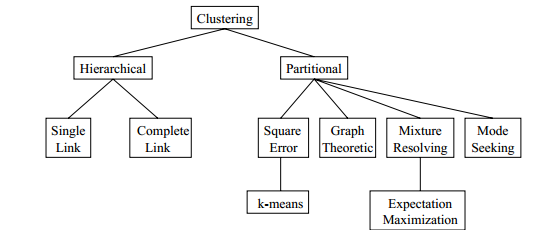
\includegraphics{./Figures/clustering.png}
		\rule{35em}{0.5pt}
	\caption[Clustering techniques]{Clustering techniques}
	\label{fig:clustering_approaches}
\end{figure}

\begin{itemize}
\item{Partitional : Given a database of objects, a partitional clustering algorithm constructs
partitions of the data, where each cluster optimizes a clustering criterion, such as the minimization of the sum of squared distance from the mean within each cluster.
One of the issues with such algorithms is their high complexity, as some of them exhaustively enumerate
all possible groupings and try to find the global optimum. Even for a small number of objects,
the number of partitions is huge. That’s why, common solutions start with an initial, usually
random, partition and proceed with its refinement. A better practice would be to run the partitional algorithm for different sets of initial points (considered as representatives) and investigate whether all solutions lead to the same final partition.
Partitional Clustering algorithms try to locally improve a certain criterion. First, they compute the
values of the similarity or distance, they order the results, and pick the one that optimizes the criterion.Hence, the majority of them could be considered as greedy-like algorithms.}

\item{Hierarchical algorithms create a hierarchical decomposition of the objects. They are either
agglomerative (bottom-up) or divisive (top-down):
\begin{itemize}
\item{Agglomerative algorithms start with each object being a separate cluster itself, and successively
merge groups according to a distance measure. The clustering may stop when all objects are in
a single group or at any other point the user wants.
These methods generally follow a greedy-like bottom-up merging.}
\item{Divisive algorithms follow the opposite strategy. They start with one group of all objects and
successively split groups into smaller ones, until each object falls in one cluster, or as desired.
Divisive approaches divide the data objects in disjoint groups at every step, and follow the same
pattern until all objects fall into a separate cluster. This is similar to the approach followed by
divide-and-conquer algorithms.
Partitional and hierarchical methods can be integrated. This would mean that a result given by a hierarchical
method can be improved via a partitional step, which refines the result via iterative relocation
of points.
}
\end{itemize}
}
\end{itemize}
Apart from the two main categories of  partitional and hierarchical clustering algorithms, many other methods
have emerged in cluster analysis, and are mainly focused on specific problems or specific data sets
available. These methods include:
\begin{itemize}
\item
Density-Based Clustering : These algorithms group objects according to specific density objective functions.
Density is usually defined as the number of objects in a particular neighborhood of a data objects.
In these approaches a given cluster continues growing as long as the number of objects in the
neighborhood exceeds some parameter. This is considered to be different from the idea in partitional
algorithms that use iterative relocation of points given a certain number of clusters.
\item
Grid-Based Clustering : The main focus of these algorithms is spatial data, i.e., data that model the geometric
structure of objects in space, their relationships, properties and operations. The objective of
these algorithms is to quantize the data set into a number of cells and then work with objects belonging
to these cells. They do not relocate points but rather build several hierarchical levels of groups of
objects. In this sense, they are closer to hierarchical algorithms but the merging of grids, and consequently
clusters, does not depend on a distance measure but it is decided by a predefined parameter.
\item
Model-Based Clustering : These algorithms find good approximations of model parameters that best fit
the data. They can be either partitional or hierarchical, depending on the structure or model they
hypothesize about the data set and the way they refine this model to identify partitionings. They
are closer to density-based algorithms, in that they grow particular clusters so that the preconceived
model is improved. However, they sometimes start with a fixed number of clusters and they do not
use the same concept of density.
\item
Categorical Data Clustering : These algorithms are specifically developed for data where Euclidean, or
other numerical-oriented, distance measures cannot be applied. In the literature, we find approaches
close to both partitional and hierarchical methods.
\end{itemize}
%----------------------------------------------------------------------------------------
\section{Semantic Similarity}
The problem of formalizing and quantifying the intuitive notion of similarity has a long history in philosophy, psychology, and artificial intelligence, and many different perspectives have been suggested. Recent research on the topic in computational linguistics has emphasized the perspective of semantic relatedness of two lexemes in a lexical resource, or its inverse, semantic distance. It’s important to note that semantic relatedness is a more general concept than similarity; similar entities are usually assumed to be related by virtue of their likeness (bank - trust company), but dissimilar entities may also be semantically related by lexical relationships such as metonymy (car - wheel) and antonymy (hot - cold), or just by any kind of functional relationship or frequent association (pencil - paper, penguin - Antarctica).\\

Measures of text similarity have been used for a long time in applications in natural language processing and related areas. Text similarity has been also used for relevance feedback and text classification (Rocchio, 1971), word sense disambiguation (Lesk, 1986), and more recently for extractive summarization (Salton et al., 1997b), and methods for automatic evaluation of machine translation (Papineni et al., 2002) or text summarization (Lin and Hovy, 2003). \\
The typical approach to finding the similarity between two text segments is to use a simple lexical matching method, and produce a similarity score based on the number of lexical units that occur in both input segments. \\
Improvements to this simple method have considered stemming, stop-word removal, part-of-speech tagging, longest subsequence matching, as well as various weighting and normalization factors (Salton et al., 1997a).\\
While successful to a certain degree, these lexical matching similarity methods fail to identify the semantic similarity of texts. For instance, there is an obvious similarity between the text segments I own a dog and I have an animal, but most of the current text similarity metrics will fail in identifying any kind of connection between these texts. \\

The only exception to this trend is perhaps the latent semantic analysis (LSA) method (Landauer et al., 1998), which represents an improvement over earlier attempts to use measures of semantic similarity for information retrieval (Voorhees, 1993), (Xu and Croft, 1996). LSA aims to find similar terms in large text collections, and measure similarity between texts by including these additional related words. \\
However, to date LSA has not been used on a large scale, due to the complexity and computational cost associated with the algorithm, and perhaps also due to the “black-box” effect that does not allow for any deep insights into why some terms are selected as similar during the singular value decomposition process.\\

On the other hand, another group of approaches that gaines wide approval is the Knowledge-based group. Knowledge-based can be explained as a measure of semantic similarity between words, and an indication of the word specificity.\\

%----------------------------------------------------------------------------------------
\section{Recommendation}
As the World Wide Web grows, recommender systems are becoming an increasingly important aspect to all e-commerce portals. Popular purchasing sites such as Amazon (www.amazon.com) and eBay (www.ebay.com) represent some of the businesses that have integrated recommendations into their shopping experience. These systems help to overcome excess information overload by providing customers with recommendations or suggestions based on their likes and dislikes relative to other customers.
Recommendations have become an integral aspect of these e-commerce platforms and have shown to personalize the shopping experience.(Schafer, Konstan and Riedi 1999) 
\subsection{Definition of a Recommender System}
Recommender systems are a type of information filtering system that gives advice on products, information, or services that a user may be interested in. They assist users ith the decision making process when choosing items with multiple alternatives(Werthner, Hansen and Ricci 2007). Recommender systems are popular due to their e-commerce application purposes. Within the e-commerce world, recommendations provide aid to customers and help them find what they may be looking for, thus increasing business. In addition, it can be used as a tool to predict user's behavior, but should not be used to select recommendations on their behalf.
There are two basic entities that appear in any recommender system are the user and the item of interest. The user can be a customer in an e-commerce platform or an avid book reader looking for a recommendation for the next book they should read. The users provide their ratings on items and are used to aid other users with their recommendations. The item is the second piece of a recommender system. Users give items ratings and the algorithm outputs recommended items based on new user queries.
\subsection{Basics to a Recommender System}
All recommender systems, whether they are in the e-commerce world or any other application, all have three things in common: they all take in inputs; they all have a goal; and they all produce and output (Vozalis and Margaritis 2003).
The input in a recommender system can depend on the type of recommender system algorithm. Generally, inputs belong to one of the following categories:
1.Votes/Ratings: Ratings are based on the opinions of users on specific items that they have reviewed.
2.Demographic data: Information such as age, gender, education, and location of the user are factors that a recommender system can utilize.
3.Content data: textual analysis of documents related to the item that has been rated by the user. This information will also assist in the recommender system.
The goal of a recommender system is to predict what the user will rate an item or generate suggestions about these items. The goal is generated based on the input of previous users within a user-item matrix. This matrix is used to correlate users/items to the current user/item and generate a recommendation. 
Finally, the output of a recommender system can either be a prediction or the expected rating score the active user will give the current item. A recommendation is a single or list of items that have the highest prediction.
\subsection{Challenges of Recommender Systems}
\subsubsection{Quality of a recommender system}
Can the recommender system be trusted to produce accurate recommendations? The recommender system must eliminate recommendations produced by the system that the system believes the user will like but in actually the user does not like. These are also known as false positives. (Vozalis and Margaritis 2003)
\subsubsection{Sparsity}
Since users may not rate some items, the user-item matrix may have many missing ratings and be very sparse. Therefore, finding correlations between users and items becomes quite difficult and can lead to weak recommendations. (Melleville,Mooney and Nagarajan 2002)
\subsubsection{Synonymy}
Recommender systems are usually not able to discover associations between similar items that may just have different names.
\subsubsection{First Rater Problem}
An item cannot be recommended unless it has been rated before. The problem usually occurs when new items are added to the system or when there are items that are rarely viewed and therefore may not have been rated. (Melleville, Mooney and Nagarajan 2002)
\subsection{Memory Based Recommender Systems}
Recommender systems that utilize memory-based algorithms and utilize a user-item matrix to generate a prediction fall under the memory based recommender systems category. The majority of such systems belong to Collaborative Filtering (CF) systems. There are three steps into processing a recommendation based on a CF system:
1.Representation
2.Neighborhood Formation
3.Recommendation Generation
\subsubsection{User‐Based Recommendation}
A user-based recommendation system involves seeing how well users correlate to each other and using this information to derive predictions. A running example will demonstrate how a user-based recommendation can easily generate a prediction using a mathematical algorithm.
\subsubsubsection{Representation}
Since there are two aspects to a recommender system as noted above. The users and the items can be placed as a collection of numerical ratings into a user-item matrix.\\
\begin{table}[ht]
\caption{User Item Matrix} % title of Table
\centering  % used for centering table
\begin{tabular}{c c c c} % centered columns (5 columns)
\hline\hline                        %inserts double horizontal lines
 & Item1 & Item2& Item3 \\ [0.5ex] % inserts table 
%heading
\hline                  % inserts single horizontal line

John & 2 & 3  & 5  \\
Bob & 3 & 4 & 3 \\
Lucy & 5 & 2& Did not rate \\[1ex]      % [1ex] adds vertical space
\hline %inserts single line
\end{tabular}
\label{table:3} % is used to refer this table in the text
\end{table}

As seen in Table 1, a user-item matrix allows for the creation of a neighborhood that can be used to create similarity between users whom we wish to generate recommendations for. The user-item matrix is usually sparse since most users do not rate every item or may not have used the specific item.
Sparsity can be an issue that can lead to weak recommendations. Two common processes that can reduce the sparsity issue and improve the satisfaction of the recommender system are:
1.Default Voting: Setting an appropriate rating for all items that have not been rated. The cost of applying a default rating is low (Vozalis and Margaritis 2003).   - Table 1: Providing Lucy with a default value of 3 for Item 3.
2.Pre-processing using averages: Scan through missing items and either averaging user’s votes or averaging the item votes and placing the resulting average as the rating value for the missing user-item matrix entry (Vozalis and Margaritis 2003)    - Table 1: Lucy’s other items provide an average of 3.5. Therefore, we can pre-process her rating for Item 3.
\subsubsubsection{Neighbourhood Formation}
Generating a neighborhood involved calculating the similarity between the given users within the user-item matrix. Similarity will be used to generate a recommendation for a specific user.
The algorithm follows these steps:
1.Compare the similarity between all users with the active user.
2.Select n users that have the highest similarity to build a neighborhood
3.Compute the prediction based on this similarity matrix.
Within the user-based recommendation system, similarity between two users is calculated using the Pearson’s correlation coefficient. Pearson’s correlation (also called the Pearson's product moment correlation after Karl Pearsons) has become a standard way of calculating correlation.

\begin{table}[ht]
\caption{Similarity matrix based on values from Table 2.1} % title of Table
\centering  % used for centering table
\begin{tabular}{c c c c} % centered columns (5 columns)
\hline\hline                        %inserts double horizontal lines
 & John & Bob& Lucy \\ [0.5ex] % inserts table 
%heading
\hline                  % inserts single horizontal line

John & 1 & -0.1887  & -0.5146 \\
Bob &  & 1 & -0.9486 \\
Lucy &  & & 1 \\[1ex]      % [1ex] adds vertical space
\hline %inserts single line
\end{tabular}
\label{table:3} % is used to refer this table in the text
\end{table}

\subsubsubsection{Generate Prediction}
The prediction is a numerical value that represents a predicted opinion of the active user about a specific item. The prediction for a user-based collaborative filtering algorithm needs both the user-item matrix (Table 1) and the similarity matrix (Table 2).
\subsubsection{Item‐Based Recommendation}
This form of collaborative filtering is computed based on item relations and not on user relations. An item-based collaborative filtering algorithm looks at the set of items that an active user has rated and computes how similar the set of items are to the target item. Using this data, the item-based algorithm then uses the similarity and calculates the prediction based on weighted averages of the active user’s ratings on those similar items. (Sarwar, et al. 2001)
The prediction algorithm for item-based collaborative filtering follows the same procedure as the user-based collaborative filtering. Item-based collaborative filtering follows the same three procedures: representation, neighborhood formation, and prediction generation. Within representation, item-based CF uses the user-item matrix seen in Table 1. The neighborhood formation creates a similarity matrix. This  similarity matrix uses the Pearson Correlation coefficient, however, determines the correlation between two items
\subsection{Comparison between User‐based and Item‐based recommender systems}
There are two major factors that come into play when talking about how user-based recommender systems compare to item-based recommender systems - the quality of the results and the performance results. 
In an experiment performed by the GroupLens Research group, it was conclusive that based on building a user-based and an item-based recommender system, the item-based recommender system provided better quality of results with a lower MAE (Mean Accuracy Error) than the user-based recommender system(Sarwar, et al. 2001). 
In terms of performance, the GroupLens Research group has also concluded that an  item based recommender system also has better performance over a user-based system since the item neighborhood is fairly static and can potentially be pre-computed, which results in higher online performance(Sarwar, et al. 2001)
\subsection{Content‐Based Recommender Systems}
Content-based recommendation systems or content-based filtering is based on textual information such as documents. These items are typically described with keywords and weights. Using nearest neighbor functions or clustering methods can allow this recommendation system to analyze these keywords and document content and use it as a basis to recommend a suitable item. This will also be based on the items characteristics. The different techniques used in this method of information filtering follow two approaches: Heuristic-based and model-based methods. Heuristic-based methods include KNN algorithms and clustering methods while model-based methods include Bayesian filtering, artificial neural networks, and clustering. Content-based filtering systems are limited by their content. If they have limited keywords or overspecialization problems, they produce weak recommendations. (Wei, Jinghu and Shaohung 2007)
\subsection{Testing the Accuracy of a Recommender System}
There are multiple ways to evaluate the predictive quality of recommender systems. We usually evaluate a recommender system based on accuracy.
\subsubsection{Accuracy}
To measure a recommender system’s accuracy, we usually measure how effective the system’s predictions are to actual results. A common way of measuring accuracy is by using a statistical accuracy metric called Mean Accuracy Error (MAE).
\subsubsection{Mean Absolute Error}
MAE is measured for items that the user has expressed opinions and given a rating to using the following equation (Vozalis and Margaritis 2003). The recommender system has to have generated its list of predictions and the actual ratings have to be provided as well. A lower MAE corresponds to a more accurate prediction.
MAEi=j=1ni|arij-rij|ni
Where ni is the number of items that the user has expressed ratings on, rij are the predictions generated for the chosen items and arij are the actual ratings provided by the user for those chosen items.
In terms of grades, which will be the case in this study, a MAE of 5 will mean that the predicted grades are on average different from the actual grades by about 5 marks.
We can use the MAE to determine if specific sets of data to determine if the model improves as we enter more ratings for that specific user. With these tests and assessments, we can determine if our recommender system is performing well or if adjustments need to be made in order to improve accuracy.
 
\input{./Chapters/Chapter3}
% Chapter 4

\chapter{Used Semantic Similarity Measures} % Main chapter title

\label{sim} % For referencing the chapter elsewhere, use \ref{Chapter1} 

\lhead{Chapter 4. \emph{Used Similarity Measures}} % This is for the header on each page - perhaps a shortened title

%----------------------------------------------------------------------------------------

This chapter is organized as follows Section ~\ref{lexicalsim} discusses the Lexical Similarity, semantic similarity is presented in section ~\ref{semanticSim}, which discuss corpus-based semantic similarity, and knowledge based similarity.

\section{Lexical Similarity}
\label {lexicalsim}
In linguistics, lexical similarity is a measure of the degree to which the word sets of two given languages  are similar. A lexical similarity of 1 (or 100\%) would mean a total overlap between vocabularies, whereas 0 means there are no common words.\\


\subsection{Document Represenatation}
\label {documentrep}
There are several ways to model a text document. For example, it can be represented as a bag of words, where words are assumed to appear independently and the order is immaterial. The bag of word model is widely used in information retrieval and text mining . Words are counted in the bag, which differs from the mathematical definition of set. Each word corresponds to a dimension in the resulting data space and each document then becomes a  vector consisting of non-negative values on each dimension. Here we use the frequency of each term as its weight, which means terms that appear more frequently are more important and descriptive for the document.
Let $D = \{d_1 , . . . , d_n \}$ be a set of documents and $T = \{t_1 , . . . ,t_m \}$ the set of distinct terms occurring in D. We discuss more precisely what we mean by "terms" below: for the moment just assume they are words. A document is then represented as a m-dimensional vector $t_d$.\\
Let tf (d, t) denote the frequency of term $t \,\epsilon\, T$ in document $d \, \epsilon\, D$. Then the vector representation of a document d is
\begin{equation}
\vec{t_{a}} = (tf(d,t_1),.....,tf(d,t_m))
\end{equation}
Although more frequent words are assumed to be more important as mentioned above, this is not usually the case in practice. For example, words like \RL{في , و ,ان} are probably the most frequent words that appear in Arabic text, but neither are descriptive nor important for the document’s subject. In fact, more complicated strategies such as the tfidf weighting scheme is normally used instead\citep{tfidf}.
\begin{figure}[htbp]
	\centering
		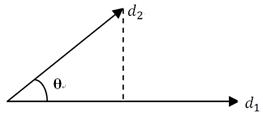
\includegraphics{./Figures/a.png}
		\rule{35em}{0.5pt}
	\caption[Angle Between Documents]{Angle Between Documents}
	\label{fig:Angle_Between_Documents}
\end{figure}
With documents presented as vectors, we measure the degree of similarity of two documents as the correlation between their corresponding vectors, which can be further quantified as the cosine of the angle between the two vectors.
Figure ~\ref{fig:Angle_Between_Documents} shows the angle in two-dimensional space but in practice the document space usually has tens and thousands of dimensions\citep{lexical}.

\subsubsection{Eculidean Distance}
\label {euclidean}
Euclidean distance is a standard metric for geometrical problems. It is the ordinary distance between two points and can be easily measured with a ruler in two- or three-dimensional space. Euclidean distance is widely used in clustering problems, including clustering text. It satisfies all the above four conditions and therefore is a true metric. It is also the default distance measure used with the K-means algorithm.\\
Measuring distance between text documents, given two documents $d_{a} and  d_{b}$ represented by their term vectors  $\overrightarrow{t_{a}} \,and\, \overrightarrow{t_{b}}$ respectively, the Euclidean distance of the two documents is defined as
where the term set is $T = {t1 , . . . , tm }$. As mentioned previously, we use the tf-idf value as term weights, that is
crucial for cluster analysis, especially for a particular type $w_{t,a} = tf idf (d_{a} , t)$.

\subsubsection{Cosine Similarity}
\label {cosine}
When documents are represented as term vectors, the similarity of two documents corresponds to the correlation between the vectors. This is quantified as the cosine of the angle between vectors, that is, the so-called cosine similarity. It is one of the most popular similarity measure applied to text documents, such as in numerous information retrieval applications and clustering too.
Given two documents $\overrightarrow{t_{a}} \,and\, \overrightarrow{t_{b}}$, their cosine similarity is

\begin{equation}
SIM_{c}(\vec{t_{a}},\vec{t_{b}}) =\frac{\vec{t_{a}}.\vec{t_{b}}}{|\vec{t_{a}}|\times|\vec{t_{b}}|}
\end{equation}

where $\overrightarrow{t_{a}} \,and\, \overrightarrow{t_{b}}$ are m-dimensional vectors over the term set $T = \{t1 , . . . , tm \}$. Each dimension represents a term with its weight in the document, which is non-negative. As a result, the cosine similarity is non-negative and bounded between [0,1].\\
An important property of the cosine similarity is its independence of document length. For example, combining two identical copies of a document $d$ to get a new pseudo document $d'$ , the cosine similarity between $d$ and $d'$ is 1, which means that these two documents are regarded to be identical. Meanwhile, given another document $l$, $d$ and $d'$ will have the same similarity value to l, that is, 
$SIM_{c}(\vec{t_{d}},\vec{t_{l}})= SIM_{c}(\vec{t_{d'}},\vec{t_{l}})$.\\ 
In other words, documents with the same composition but different totals will be treated identically. Strictly speaking, this does not satisfy the second condition of a metric,because after all the combination of two copies is a different object from the original document. However, in practice,when the term vectors are normalized to a unit length such as 1, and in this case the representation of $d$ and $d'$ is the same.

%----------------------------------------------------------------------------------------

\section{Semantic Similarity}
\label {semanticSim}
Measures of semantic similarity have been traditionally defined between words or concepts, and much less between text segments consisting of two or more words. The emphasis on word-to-word similarity metrics is probably due to the availability of resources that specifically encode relations between words or concepts (e.g. WordNet), and the various testbeds that allow for their evaluation (e.g. TOEFL or SAT analogy/synonymy tests). \\
Moreover, the derivation of a text-to-text measure of similarity starting with a word based semantic similarity metric may not be straightforward,and consequently most of the work in this area has considered mainly applications of the traditional vectorial model,occasionally extended to n-gram language models\citep{semantic}.\\

Given two input text segments, we want to automatically derive a score that indicates their similarity at semantic level,thus going beyond the simple lexical matching methods traditionally used for this task. Although we the fact that a comprehensive metric of text semantic similarity  should also take into account the structure of the text, we could model the semantic similarity of texts as a function of the semantic similarity of the component words. We do this by combining metrics of word-to-word similarity and word specificity into a formula that is a potentially good indicator of the semantic similarity of the two input texts.\\
   The following section provides details on some different corpus-based and knowledge-based measures of word semantic similarity. In addition to the similarity of words, we also take into account the specificity of words, so that we can give a higher weight to a semantic matching identified between two specific words (e.g. collie and sheepdog), and give less importance to the similarity measured between generic concepts 
(e.g. get and become).\\
Given a metric for word-to-word similarity and a measure of word specificity, we define the semantic similarity of two text segments $T1$ and $T2$ using a metric that combines the semantic similarities of each text segment in turn with respect to the other text segment. First, for each word $w$ in the segment $T1$ we try to identify the word in the segment $T2$ that has the highest semantic similarity $(maxSim(w, T2 ))$, according to one of the word-to-word similarity measures described in the following section~\ref{measuresSection}. Then, the same process is applied to determine the most similar word in $T1$ starting with words in $T2$ . The word similarities are then weighted with the corresponding word specificity, summed up, and normalized with the length of each text segment. Finally the resulting similarity scores are combined using a simple average. Note that only open-class words and cardinals can participate in this semantic matching process. As done in previous work on text similarity using vector-based models, all function words are discarded.
The similarity between the input text segments $T_1$ and $T_2$ is therefore determined using the following scoring function:
    
\begin{equation}
\label{simEq}
SIM({T_{1}},{T_{2}}) =\frac{1}{2}(\frac{\sum_{w\in \{T_1\}} (maxSim(w,T_2 * idf(w)))}{\sum_{w\in \{T_1\}} idf(w)} + \frac{\sum_{w\in \{T_2\}} (maxSim(w,T_1 * idf(w)))}{\sum_{w\in \{T_2\}} idf(w)})
\end{equation}

   This similarity score has a value between 0 and 1, with a score of 1 indicating identical text segments, and a score of 0 indicating no semantic overlap between the two segments.Note that the maximum similarity is sought only within classes of words with the same part-of-speech. The reason behind this decision is that most of the word-to-word knowledge-based measures cannot be applied across parts-of-speech, and consequently, for the purpose of consistency,we imposed the “same word-class” restriction to all the word-to-word similarity measures. This means that, for instance, the most similar word to the noun flower within the text “There are many green plants next to the house” will be sought among the nouns plant and house, and will ignore the words with a different part-of-speech (be, green, next). Moreover, for those parts-of-speech for which a word-to-word semantic similarity cannot be measured (e.g. some knowledge-based measures are not defined among adjectives or adverbs), we use instead a lexical match measure,which assigns a maxSim of 1 for identical occurrences of a word in the two text segments.
\subsection{Similarity Measures}
\label {SimilarityMeasures}
\label{measuresSection}
The Leacock \& Chodorow (Leacock \& Chodorow 1998) similarity is determined as:
\begin{equation}
SIM_{lch} = -log \frac{length}{2 \times D}
\end{equation}
where length is the length of the shortest path between two concepts using node-counting, and D is the maximum depth of the taxonomy.
The Lesk similarity of two concepts is defined as a function of the overlap between the corresponding definitions, as provided by a dictionary. It is based on an algorithm proposed by Lesk (1986) as a solution for word sense disambiguation.
The application of the Lesk similarity measure is not limited to semantic networks, and it can be used in conjunction with any dictionary that provides word definitions.
The Wu and Palmer (Wu \& Palmer 1994) similarity metric measures the depth of two given concepts in the WordNet taxonomy, and the depth of the least common subsumer (LCS), and combines these figures into a similarity score:
\begin{equation}
SIM_{wup} =\frac{2\times depth(LCS)}{depth(concept1) + depth(concept2)}
\end{equation}
The measure introduced by Resnik (Resnik 1995) returns the information content (IC) of the LCS of two concepts:
\begin{equation}
Sim_{res} = IC(LCS)
\end{equation}
where $IC$ is defined as:
$IC(c) = -log P(c)$ and $P(c)$ is the probability of encountering an instance of concept c in a large corpus.
The next measure we use in our experiments is the metric introduced by Lin (Lin 1998), which builds on Resnik’s measure of similarity, and adds a normalization factor consisting of the information content of the two input concepts:
\begin{equation}
SIM_{wup} =\frac{2\times IC(LCS)}{IC(concept1) + IC(concept2)}
\end{equation}
Finally, the last similarity metric considered is Jiang \& Conrath (Jiang \& Conrath 1997):
\begin{equation}
SIM_{jnc} =\frac{1}{IC(concept1) + IC(concept2) - 2\times IC(LCS)}
\end{equation}
Note that all the word similarity measures are normalized so that they fall within a 0–1 range. The normalization is done by dividing the similarity score provided by a given measure with the maximum possible score for that measure. 

\subsection{Corpus Based}
\label {corpus}
\subsubsection{LSA for Semantic Similarity}
LSA is a fully automatic mathematical/statistical technique for extracting and inferring relations of expected contextual usage of words in passages of discourse. It is not a traditional natural language processing or artificial intelligence program; it uses no humanly constructed dictionaries, knowledge bases, semantic networks, grammars, syntactic parsers, or morphologies, or the like, and takes as its input only raw text parsed into words defined as unique character strings and separated into meaningful passages or samples such as sentences or paragraphs.
Another way to think of this is that LSA represents the meaning of a word as a kind of average of the meaning of all the passages in which it appears, and the meaning of a passage as a kind of average of the meaning of all the words it contains. LSA's ability to simultaneously derive representations of these two interrelated kinds of meaning depends on an aspect of its mathematical machinery.\\

A rough analogy of how this can happen is as follows. Read the following sentence:\\
"John is Bob's father and Mary is Ann's mother." Now read this one: "Mary is Bob's mother."\\
Because of the relations between the words mother, father, son, daughter, brother and sister that you already knew, adding the second sentence probably tended to make you think that that Bob and Ann were brother and sister, Ann the daughter of John, John the father of Ann, and Bob the son of Mary, even though none of these relations is explicitly expressed (and none follow necessarily from the presumed formal rules of English kinship naming.) The relationships inferred by LSA are also not logically defined, nor are they assumed to be consciously rationalizable as these could be. Instead, they are relations only of similarityãor of context sensitive similarityãbut they nevertheless have mutual entailments of the same general nature, and also give rise to fuzzy indirect inferences that may be weak or strong and logically right or wrong\citep{lsa}.

\paragraph{How LSA works}
The first step is to represent the text as a matrix (the term-by-document matrix T)in which each row stands for a unique word and each column stands for a text passage or other context. Each cell contains the frequency with which the word of its row appears in the passage denoted by its column. Next, the cell entries are subjected to a preliminary transformation, whose details we will describe later, in which each cell frequency is weighted by a function that expresses both the word's importance in the particular passage and the degree to which the word type carries information in the domain of discourse in general.
Next, LSA applies singular value decomposition (SVD) to the matrix. This is a form of factor analysis, or more properly the mathematical generalization of which factor analysis is a special case. In SVD, a rectangular matrix is decomposed into the product of three other matrices. One component matrix (U) describes the original row entities as vectors of derived orthogonal factor values, another (V) describes the original column entities in the same way, and the third is a diagonal matrix (SIGMA) containing scaling values such that when the three components are matrix-multiplied, the original matrix (T) is reconstructed. 
There is a mathematical proof that any matrix can be so decomposed perfectly, using no more factors than the smallest dimension of the original matrix. When fewer than the necessary number of factors are used, the reconstructed matrix is a least-squares best fit. 

One can reduce the dimensionality of the solution simply by deleting coefficients in the diagonal matrix (SIGMA), ordinarily starting with the smallest. (In practice, for computational reasons, for very large corpora only a limited number of dimensions, currently a few thousands can be constructed). The SVD equations can be derived as follows\citep{lsa}:\\
\begin{equation}
\{X\} = \{W\}\{S\}\{P\}^T
\end{equation}

\paragraph{Stop-listing and stemming}
These are very rarely used. In keeping with the underlying theory and model, neither stemming nor stop-listing is appropriate or usually effective. As in natural language, the meaning of passages cannot be accurately reconstructed or understood without all of its words. However, when LSA is used to compare word strings shorter than normal text paragraphs, e.g. short sentences, zero weighting of function words is often pragmatically useful.
\paragraph{Similarity in the reduced space}
Since both passages (documents) and terms (words) are represented as vectors, it is straight forward to compute the similarity between passage-passage, term-term, and term-passage. In addition, terms and/or passages can be combined to create new vectors in the space. The process by which new vectors can be added to an existing LSA space is called folding-in. The cosine distance between vectors is used as the measure of their similarity for many applications because of its relation to the dot-product criterion and has been found effective in practice, although other metrics, such as Euclidean distance or City-Block (Manhattan) distance are sometimes used.

\paragraph{Shortfalls, objections, evidence and arguments}
potential limitations should be noted:
\begin{itemize}
\item [1.] It is likely, of course, that LSA's “bag of words” method, that ignores all syntactical, logical and nonlinguistic pragmatic entailments, sometimes misses meanings or gets it scrambled.
\item[2.] LSA became practical only when computational power and algorithm efficiency improved sufficiently to support SVD of thousands of words-by-thousands of contexts matrices; it is still impossible to perform SVD on the hundreds of thousands by tens of millions matrices that would be needed to truly represent the sum of an adult's language exposure.
\end{itemize}
Some commentators have also argued that LSA must be fundamentally wrong as theory because is not grounded in perception and intention. The strength of this objection is considerably reduced by the observation that language must veridically reflect these sources or it would be nearly useless, and by the human ability to generate, use and understand words as abstract and unrelated to perception as the word abstract itself, and by LSA’s varied successes.

Indeed, one should not think of LSA as a fixed mechanism or its representations as
fixed quantities, but rather, as evolving approximations.
%-------------------------------------------------------------------------------
\subsection{Knowledge Based}
\label {knowledge}
Evaluating semantic relatedness using network representations is a problem with a long history in artificial intelligence and psychology, dating back to the spreading activation approach of Quillian (1968) and Collins and Loftus (1975). Semantic similarity represents a special case of semantic relatedness: for example, cars and gasoline would seem to be more closely related than, say, cars and bicycles, but the latter pair are certainly more similar.\\
Rada et al.\citep{rada1989development} suggest that the assessment of similarity in semantic networks can in fact be thought of as involving just taxonomic (is-a) links, to the exclusion of other link types; that view will also be taken here, although admittedly links such as part-of can also be viewed as attributes that contribute to similarity.\\
    A natural, time-honored way to evaluate semantic similarity in a taxonomy is to measure the distance between the nodes corresponding to the items being compared - the shorter the path from one node to another, the more similar they are. Given multiple paths, one takes the length of the shortest one.\\
    A widely acknowledged problem with this approach, however, is that it relies on the notion that links in the taxonomy represent uniform distances. Unfortunately, uniform link distance is difficult to define, much less to control. In real taxonomies, there is wide variability in the "distance" covered by a single taxonomic link, particularly when certain sub-taxonomies (e.g., biological categories) are much denser than others. For example, in WordNet, broad-coverage semantic network for English, it is not at all difficult to find links that cover an intuitively narrow distance (rabbit ears is-a television antenna) or an intuitively wide one (phytoplankton is-a living thing). The same kinds of examples can be found in the Collins COBUILD Dictionary (Sinclair, ed., 1987), which identi es superordinate terms for many words (e.g.,safety valve is-a valve seems much narrower than knitting machine is-a machine)\citep{semantic_2}.\\

\subsubsection{AWN}
AWN is constructed according to the methods developed for EuroWordNet (EWN;Vossen 1998) and since applied to dozens of languages around the world. The EuroWordNet approach maximizes compatibility across wordnets and focuses on manual encoding of the most complicated and important concepts\citep{awn_0}. \\
Language-specific concepts and relations are encoded as needed or desired. This results in a so-called core wordnet for Arabic with the most important synsets, embedded in a solid semantic framework. From this core wordnet, it is possible to automatically extend the coverage with high precision. Specific concepts can be linked and translated with great accuracy because the base building blocks are manually defined and translated. \\
The approach follows a top-down procedure. Arabic Base Concepts are defined and extended via hyponymic relations to derive a core wordnet. The set of Common Base Concepts (CBCs) from the 12 languages in EWN and BalkaNet (Tufis 2004) are encoded as synsets; other language-specific concepts are added and translated manually to the closest synset(s) in Arabic. The same step is performed for all English synsets that currently have an equivalence relation in Suggested Upper Merged Ontology (SUMO).\\
The first layers of hyponyms are chosen on the basis of linguistic and applications based criteria; the final phase completes the target set of concepts/synsets, including specific domains and named entities. Each synset construction step is followed by a validation phase, where formal consistency is checked and the coverage is evaluated in terms of frequency of occurrence and domain distribution.\\

\paragraph{Structure and organization of AWN}
Because AWN is to be aligned not just to Princeton WordNet (PWN) (Fellbaum 1998) but to every wordnet aligned to PWN, the database design supports multiple languages, and the user interface will be explicitly multilingual rather than bilingual as was the one described in Black and Elkateb (2004)\citep{awn_1}.
The database structure comprises four principal entity types, item, word, form and link.
\begin{itemize}
\item [1.] Items are conceptual entities, including synsets, ontology classes and instances. Besides a unique identifier, an item has descriptive information such as a gloss. Items lexicalized in different languages are distinct.
\item [2.]A word entity is a word sense, where the citation form of the word is associated with an item via its identifier.
\item [3.]A form is a special form that is considered dictionary information (not merely an inflectional variant). The forms of Arabic words that go in this table are the root and/or the broken plural form, where applicable.
\item [4.]A link relates two items, and has a type such as "equivalence," "subsuming," etc. Links connect sense items to other sense items, e.g. a PWN synset to an AWN synset, a synset to a SUMO concept, etc.
\end{itemize}
This data model has been specified in XML as an interchange format, but is also implemented in a MySQL database hosted by one of the partners. The database will be the primary deliverable of the project, and will be distributed freely to the community.

\paragraph{Constructing AWN}
The basic criteria for selecting synsets to be covered in AWN are\citep{awn_2}: 
\begin{itemize}
\item Connectivity: AWN should be as densely connected as possible by hyperonymy / hyponymy chains, etc. Most of the synsets of AWN should correspond to English WN counterparts and the overall topology of both wordnets should be similar.
\item Relevance: Frequent and salient concepts have priority. Criteria will include the frequency of lexical items (both in Arabic and English) and the frequency of Arabic roots in their respective reference corpora.
\item Generality: Synsets on the highest levels of WN are preferred. These criteria suggest two ways for proceeding:
\item From English to Arabic: Given an English synset, all corresponding Arabic variants (if any) will be selected.
\item From Arabic to English: Given an Arabic word, all its senses have to be found, and for each of these senses the corresponding English synsets have to be selected.
\end{itemize}

Both steps have to be followed throughout the construction of AWN. All AWN synsets must be manually validated (and eventually locked, when all their variants have been found) but advantage should be taken as much as possible of the available resources for guiding the construction and validation process. Once a new Arabic verb is added to AWN, several possibilities for extension arise: extensions from verbal entries, including verbal derivatives, nominalizations, verbal nouns, etc. We also consider the most productive forms of deriving broken plurals. This can be done using a set of lexical and morphological rules. To take full advantage of these extensions short iterations will be performed. As stated in the introduction, the starting point of AWN is the manual construction of its Base Concept (BC) set from EWN and BalkaNet's CBCs. We concentrate on the most relevant terms for obtaining about 1,000 nominal and 500 verbal synsets. \\
The second step consists of the top-down vertical extension of BC, following Farreres 2005, Diab 2004). Some preprocessing is required for this and the next phase. We mention two tasks, preparation and extension. Preparation includes the processing of the available bilingual resources and the compilation of a set of lexical and morphological rules. From the set of available bilingual dictionaries we construct a homogeneous bilingual dictionary (HBIL) that contains for each entry information on the Arabic/English word pair, the Arabic root (added manually), POS, relative frequencies and sources supporting the pairing\citep{awn_2}.\\
The set of 17 heuristic methods used in the development of EWN will be applied to HBIL to derive candidate Arabic words/English synsets mappings. For each mapping the information attached includes the Arabic word and root, the English synset, POS, relative frequencies, mapping score, absolute depth in WN, number of gaps between the synset and the top of the WN hierarchy, and sources containing the pair.
Arabic words in bilingual resources must be normalized and lemmatized (Diab et al. 2004, Habash and Rambow 2005) but vowels and diacritics must be maintained. Arabic roots are not vowelized.
Following pre-processing, the set of scored Arabic word/English synset pairs becomes the input to the manual validation step. We proceed by chunks of related units (sets of related WN synsets, e.g. hyponymy chains and sets of related Arabic words, i.e., words having the same root) instead of individual units (synsets, senses, words).\\

\paragraph{Shortfalls of AWN:}
\begin{itemize}
\item High Coupling with UI\\
AWN suffers a very poor design that resulted in a high coupling between the Core Module and the Graphical User Interface (GUI) of the AWN, which made it very difficult to use the code module and the database without the GUI. However, we managed to decouple the GUI from the core modules of the AWN to allow its integration with other modules of semantic similarity. The decoupling process exerted a lot of time tracing and reverse engineering the code.
\item shortage of unique terms/word i.e there is so little number of words in database\\
       One reasonable limitation of AWN, assuming it is an initial version, is that it doesn’t contain a broad collection of Arabic words and terms. It contains only 17561 unique word, distributed among 7822 synsets.This leads to a lot of missing words that have no record in AWN’s database. e.g. \RL{جنوب افريقيا, أحمد, محمد}
\item Running time is major problem\\
Since AWN depends on the Tree Concept (a hierarchical organization of the synsets), it has an arabic tree with nodes that represent synsets, each synset contains set of words. So every time the AWN is queried by a term, in order to retrieve its synset, the whole tree is first searched for this term. If the term was not found in the tree, we seek it from database. If the term is found in the database, then the retrieved results from the database would include the path of the term in the hierarchical tree. The final step, that is to expand the retrieved path into the tree, exhausts a substantial amount of time. The time consumption is due to the way the path expansion work. \\
The path expansion starts at the tree root node and traverses the tree through the path retrieved from the database. If a node on the path was not found in the current tree, the node is added to the tree and all its children are fetched from the database and added to the tree. The last step consumes a lot of time because it expands all the node’s children, although only one child is needed. This caused the tree expansion for some words to consume up to 15 minutes.\\
Another issue that consumes a lot of time is the path retrieval from the database. When a term needs to be fetched from the database, first its synset needs to be find. After the synset is found, the path of the synset in the hierarchical tree also needs to be found. The path is assembled starting from the term’s synset traversing its parent up until the root is reached (you can think of the process traversing up the tree using Forwarding Pointers). \\
\item Bugs in the code\\
\begin{itemize}
\item There was missing logic in the code probably because these methods were never called by the GUI.
\item There was some missing constants in the core of AWN, it can't recognize some patterns of words
\end{itemize}
\end{itemize}
  
\paragraph{What we have done}
\begin{itemize}
\item We managed to decouple the Code module from the GUI to be able to use each one separately.
\item We fixed some bugs in the code.
\begin{itemize}
\item Missing logic in the code
\item Missing constants
\end{itemize}
\item we modified the expansion algorithm and managed to reduce expansion time to 20\% of the original running time.
\end{itemize}

\textit{How we Use it?}\\
\textit{Wu and Palmer}\\
    If words can be defined with concepts in a hierarchical structure, it is possible to measure the meaning similarity between words with an information measure based on WordNet (Resnik,1993), or structure level information based on a thesaurus (Kurohashi and Nagao, 1992). How-
ever, verb meanings are difficult to organize in a hierarchical structure.\\
In each conceptual domain, lexicalized concepts can be organized in a hierarchical structure. Within one conceptual domain, the similarity of two concepts is defined by how closely they are related in the hierarchy, i.e., their structural relations.\\
The Wu and Palmer \citep{wu} similarity metric measures the depth of two given concepts in the WordNet taxonomy, and the depth of the least common subsumer (LCS), and combines these figures into a similarity score:
\begin{equation}
\label{wu_palmer}
SIM({T_{1}},{T_{2}}) =\frac{2 * depth(LCS)}{depth(concept_1)+ depth(concept_2)} 
\end{equation}

so we utilized the Wu\&Palmer Technique and AWN to measure the semantic similarity according to the following stpes:
\begin{itemize}
\item [1.] Search for both terms in the Arabic Tree in the AWN if found get there’s  depth and their least common ancestor.
\item [2.] if not found search database to get their synsets and expand them in the tree. This is the most expensive operation in the whole procedure due to the database request also due to the expansion operation.
\item [3.] then get the depths of both synsets and their least common ancestor 
\item [4.] Finally use Wu and Palmer to get the similarity using the Wu and Palmer equation ~\ref{wu_palmer}
\item [5.] Apply the semantic similarity equation ~\ref{simEq}
\end{itemize}

\subsubsection{Wikipedia}
Using the traditional approach of a controlled, designed ontology has many disadvantages beginning with the often difficult task of designing and implementing the ontology. Once that it done, it must be maintained and modified, an important process in domains where the underlying concepts are evolving rapidly. ACM’s CCS, for example, undergoes periodic reorganization and redesign and yet as a classification of computer science concepts, it always seems to be out of date or even quaint. As a final problem, consider the process a person must follow in assigning ontology terms to a document. She has to be familiar with all of the possible choices or have some way to browse or search through them. She has to understand what each of the terms means, either the original meaning intended by the ontology designer or the possibly different current meaning as used by her community. Finally, she has to select the best set of terms from among the many relevant choices the ontology may present to her. The use of an implicit ontology emerging from the tagging choices of a community of individuals solves some of these problems, but also has significant disadvantages\citep{wiki_1}.\\
Some of these are inherent and others are being addressed in the research community and may ultimately admit good solutions. These problems are worth addressing because the result will be an ontology that 
\begin{itemize} \item [(1)] represents a consensus view of a community of users and \item [(2)]  is constructed and maintained by the community without cost to any organization. 
\end{itemize}
It remains unclear how the terms in such an ontology should be organized structurally, understood informally by end users, or mapped to a more formal ontology such as Cyc (Lenat 1995) or popular Semantic Web ontologies like FOAF (Ding et al. 2005). 
We are developing a system that is a blend of the two approaches based on the idea of using Wikipedia as an ontology. Specifically, each non-administrative Wikipedia page is used as a term in an ontology. These include Wikipedia articles describing individuals (Alan Turing), concepts (Emissions trading), locations (Barbados), events (collapse of the World trade Center), and categories (microbiology). 
Using Wikipedia as an ontology has many advantages: it is broad and fairly comprehensive, of generally high quality, constructed and maintained by tens of thousands of users, evolves and adapts rapidly as events and knowledge change, and free and “open sourced”. Moreover, the meaning of any term in the ontology is easy for a person to understand from the content on the Web page. Finally, the Wikipedia pages are already linked to many existing formal ontologies through efforts like DBpedia (Auer et al. 2007) and Semantic MediaWiki (Krotzsch et al. 2006) and in commercial systems like Freebase and Powerset.\\
The underlying concept of an article cannot be assessed by merely considering the words that appear in that article, in addition to that, finding out if two articles are conceptually related is an even more challenging problem and requires a lot of background domain knowledge, common sense as well as information about the context. Humans have the inborn ability to relate concepts semantically however it is still a very difficult problem for computers, which can be made easier by augmenting background domain knowledge for such tasks, which would certainly improve the accuracy and quality of prediction. Wikipedia proves to be an invaluable source for such background domain knowledge.\\

Wikipedia is a freely available online encyclopedia developed by a community of users. Wikipedia is growing exponentially and new content is being added to it daily by users around the globe. This encyclopedia comprises of millions of articles. The corpus is composed of several collections in different languages such as: English, French, German, Dutch, Chinese, Spanish, Arabic and Japanese. \\
Each collection is a set of XML documents built using Wikipedia. Documents of the Wikipedia XML collections are organized in a hierarchy of categories defined by the authors of the articles. The Wikipedia category and article network has been studied in detail with respect to different graph properties. The Wikipedia category system is a taxonomy for arranging articles into categories and subcategories.\\
However, this taxonomy is not a strict hierarchy or tree of categories, but allows multiple categorizations of topics simultaneously, i.e., some categories might have more than one super-category. It is shown that Wikipedia’s category system is a thesaurus that is collaboratively developed and used for indexing Wikipedia articles (Voss 2006). The articles within Wikipedia are inter-linked. However, these links do not impose any subcategory or super-category relationships. It has been observed that the Wikipedia article links graph generally resembles the World Wide Web graph.\\

\paragraph{Lucene}
We used lucene to buuild an inverted index on whole Wikipedia Articles, so we could be able to search for any term within the wikipedia aricles efficiently, aslo to get the search results ranked according to the search query.\\
Here is some Sample code for how we used Lucene the following one is sample indexing code, where Document object represents Wikipedia Articles to be indexed, Also ArabicAnalyzer is the Analyzer we used as it uses the light stemmer as we do in the datasets we used in our experiments.\\

\lstset{ %
  language=Java,                % the language of the code
  basicstyle=\footnotesize,           % the size of the fonts that are used for the code
  numbers=left,                   % where to put the line-numbers
  numberstyle=\tiny\color{gray},  % the style that is used for the line-numbers
  stepnumber=2,                   % the step between two line-numbers. If it's 1, each line 
                                  % will be numbered
  numbersep=5pt,                  % how far the line-numbers are from the code
  backgroundcolor=\color{white},      % choose the background color. You must add \usepackage{color}
  showspaces=false,               % show spaces adding particular underscores
  showstringspaces=false,         % underline spaces within strings
  showtabs=false,                 % show tabs within strings adding particular underscores
  frame=single,                   % adds a frame around the code
  rulecolor=\color{black},        % if not set, the frame-color may be changed on line-breaks within not-black text (e.g. commens (green here))
  tabsize=2,                      % sets default tabsize to 2 spaces
  captionpos=b,                   % sets the caption-position to bottom
  breaklines=true,                % sets automatic line breaking
  breakatwhitespace=false,        % sets if automatic breaks should only happen at whitespace
  title=\lstname,                   % show the filename of files included with \lstinputlisting;
                                  % also try caption instead of title
  keywordstyle=\color{blue},          % keyword style
  commentstyle=\color{dkgreen},       % comment style
  stringstyle=\color{mauve},         % string literal style
  escapeinside={\%*}{*)},            % if you want to add a comment within your code
  morekeywords={*,...}               % if you want to add more keywords to the set
}
\begin{lstlisting}
MaxFieldLength mlf = MaxFieldLength.UNLIMITED;
ArabicAnalyzer analyzer = new ArabicAnalyzer(Version.LUCENE_35);
IndexWriter writer = new IndexWriter(directory, analyzer, true, mlf);
Document doc;
doc = new Document();
doc.add(new Field("url", br.readLine(),	Field.Store.YES,Field.Index.NOT_ANALYZED));
doc.add(new Field("title", line,Field.Store.YES,Field.Index.ANALYZED, Field.TermVector.YES));
doc.add(new Field("contents", br.readLine(),Field.Store.YES,Field.Index.ANALYZED, Field.TermVector.YES));
writer.addDocument(doc);
writer.close();
\end{lstlisting}

While this code Snippet represents sample for searching the inverted index for a certain term that occured in the Contents of any document in the inverted index.\\

\begin{lstlisting}
IndexReader reader = IndexReader.open(new SimpleFSDirectory(new File("Index")));
TermDocs documents;
Term term = new Term("contents", doc[i]);
documents = reader.termDocs(term);
reader.docFreq(term);
documents.read(docs, freqs);
\end{lstlisting}

We downloaded the Wikipedia XML snapshot of 21 June 2011 and extracted around 450,000 Wikipedia articles. The text of each article was indexed using the Lucene text search engine library \citep{lucene} under the standard configuration. We also downloaded the Wikipedia database tables in order to create the category links graph and the article links graph.\\
\begin{figure}[htbp]
	\centering
		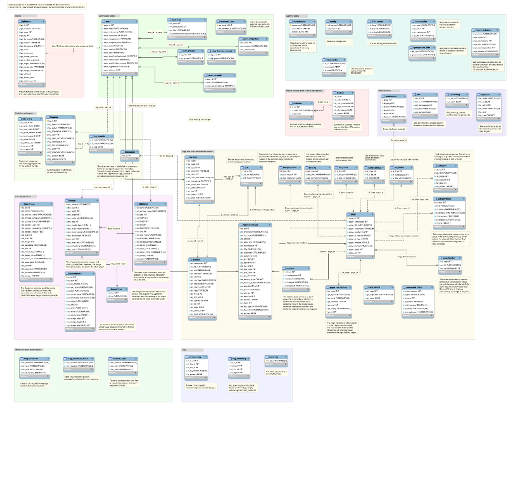
\includegraphics{./Figures/wiki_DB.png}
		\rule{35em}{0.05pt}
	\caption[Wikipedia Database Schema]{Wikipedia Database Schema}
	\label{fig:Wikipedia Database}
\end{figure}
\textit{How we Use it}\\
We have managed to implement two techniques based on the wikipedia structure as an Ontology, First technique we treated the Wikipedia Articles as Concepts\citep{wiki_1},then Every Document is represented with a vector containg around 450,000 concepts.
For each term $w_i$ in document $d_1$ we search the wikipedia articles using the inverted index built by Lucene ~\ref{luceneTool} and get vector of Articles or Concepts $V = \{c_1,c_2,...,c_n\}$, for every result lucene returns $c_i$, this term $w_i$ votes for every Article (concept  vector $V$ in the document vector where it was found by the $TF-IDF$ value in this Article.
finally we have a vetocr $d =\{\sum_{i=0}^{N} tfidf(w_1,c_i),\sum_{i=0}^{N} tfidf(w_2,c_i),...\sum_{i=0}^{N} tfidf(w_n,c_i)\} $ that represents each document we have then we apply cosine similarity to these vectors to calculate similarities ~\ref{cosine}.\\
\begin{figure}[htbp]
	\centering
		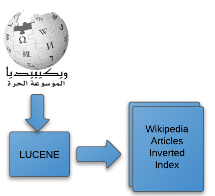
\includegraphics{./Figures/wiki_1.png}
		\rule{35em}{0.05pt}
	\caption[Wikipedia Indexing]{Wikipedia Indexing}
	\label{fig:Indexing}
\end{figure}

\begin{figure}[htbp]
	\centering
		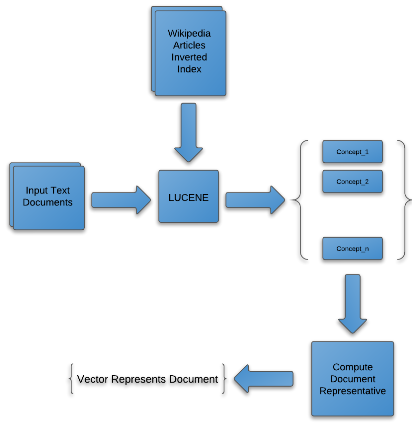
\includegraphics{./Figures/wiki_3.png}
		\rule{35em}{0.05pt}
	\caption[Wikipedia Method one]{Wikipedia Method one}
	\label{fig:Method one}
\end{figure}

\paragraph{Drawbacks}	
\begin{itemize}
\item High Dimensionality may lead to inaccurate or even incorrect results due to the sparse vectors comparison.
\item Long Running time, however it's not too long like the AWN-based Technique. 
\end{itemize}
To Overcome these problems we faced we tried two improvments on this technique, first we tried to compute the global uniopn vector for each dataset we used in the experiments to truncate those concepts that never appeared in our dataset to avoid any misleading values.With this modification only we managed to reduce the 450,000 concepts to around 8600 concepts.\\
second we applied the PCA ~\ref{pca} to reduce the high dimensionality, however this technique introduced another problem that PCA matrix result from the decomposition may contains negative values leading to negative similarities values.
To solve this new problem we tried the Automated contrast Adjustment Technique \citep{acadjstment} a used the folowing equation to map the range [-1,1] of cosine probable output and the desired range [0,1].
\begin{equation}
f(a) =a_{min}+ (a- a_{low})\times \frac{a_{max}-a_{min}}{a_{high} - a_{low}}
\end{equation}

Concerning Second Approach using the Wikipedia,We utilized the wikipedia Database ~\ref{wiki_DB} and used the categories each articles belongs to to be our concepts instead of the Article it'self. Our scoring scheme was simply count the number of times that each Wikipedia category was associated with one of the N results returned by lucene ~\ref{lucene} inverted index \citep{wiki_2}.
\begin{figure}[htbp]
	\centering
		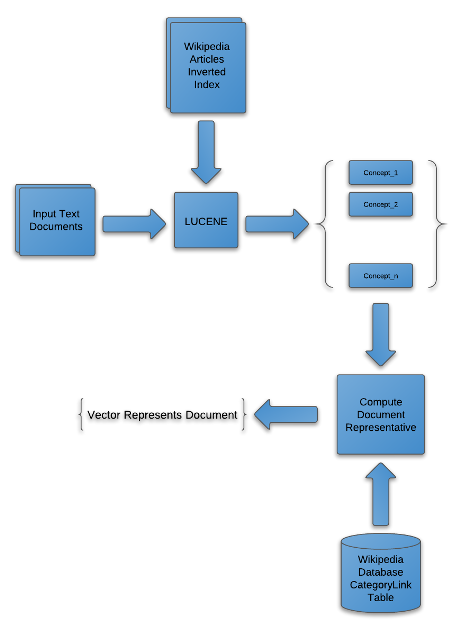
\includegraphics{./Figures/wiki_2.png}
		\rule{35em}{0.05pt}
	\caption[Wikipedia Method Two]{Wikipedia Method Two}
	\label{fig:Method Two}
\end{figure}
\subsection{Term Weigthing using Specificity}
The following section provides more insight into term Specificity, which is the idea that some words carry more semantic content than others which is also referred to as Semantic Informativeness. Computational estimation of this quantity, term specificity, is important for various applications such as information retrieval. Here in addition to the similarity of words, we also take into account the specificity of words, so that we can give a higher weight to a semantic matching identified between two specific words (e.g. collie and sheepdog), and give less importance to the similarity measured between generic concepts (e.g. get and become).\\
 While the specificity of words is already measured to some extent by their depth in the semantic hierarchy, we are reinforcing this factor with a corpus-based measure of word specificity, based on distributional information learned from large corpora.
We use two methods of computing term specificity. The first method based on modeling the rate of learning of word meaning in Latent Semantic Analysis (LSA), LSA-Specificity. The second method is TF/IDF-Specificity\citep{spec}.

\subsubsection{Latent Semantic Analysis:}
In the following section we explain using Latent Semantic Analysis for approximating term Informativeness. Latent Semantic Analysis (LSA) is a language model that represents semantic word meaning as vectors in high-dimensional space. Word vectors are positioned in such a way that semantically-related words vectors point in similar directions or have a smaller angle / higher cosine between them. The representation is derived in an unsupervised manner, by observing occurrence patterns of words in a large corpus of natural language documents. Singular Value Decomposition (SVD) on the matrix of word/document occurrence counts is used to derive the optimal set of dimensions of the space in which all of the words can be represented as vectors. The number of dimensions is then artificially reduced to a smaller number (typically around 300) of most important dimensions, which has the effect of smoothing out incidental relationships and preserving significant ones between words. The resulting geometric space allows for straightforward representation of meaning of words and/or documents; the latter are simply a weighted geometric composition of constituent word vectors. Similarity in meaning between a pair of words or documents can be obtained by computing the cosine between their corresponding vectors. For details of LSA, please see (Landauer et al., 2007), and others.\\
LSA applications almost always focus on computing the semantic similarity between words (terms). However, another property of LSA, that has a significant effect, is the term vector length. The vector length plays a very important role in many LSA calculations, in particular – in giving relative weights to the word vectors that constitute a particular text passage. As (Kintsch, 2001) wrote, “Intuitively, the vector length tells us how much information LSA has about this vector. [...] Words that LSA knows a lot about (because they appear frequently in the training corpus [...]) have greater vector lengths than words LSA does not know well. Function words that are used frequently in many different contexts have low vector lengths -- LSA knows nothing about them and cannot tell them apart since they appear in all contexts”.
The metric of term Informativeness, or specificity, which we call LSAspec, is simply the ratio of LSA word vector length to the number of documents in the LSA training corpus that contain a particular word;
\begin{equation}
LSAspec(w)=\frac{\| \overrightarrow{w}\|}{df_w}
\end{equation}
The value can be interpreted as the rate of vector length growth. We argue that more specific, or informative, words have the greatest rate of vector length growth; LSA learns about their meaning faster, with relatively fewer exposures. To illustrate this concept, let's look at a few examples that were obtained by controlling the number of occurrences of a particular word in the LSA training corpus. \\
@Mohsen: Should provide a graph for the relation of Vector lengths for some words vs. the number of documents containing those words.\\

\subsubsection{Inverse Document Frequency:}
The specificity of a word is determined using the inverse document frequency (IDF) introduced by (Sparck-Jones, 1972), defined as the total number of documents in the corpus divided by the total number of documents including that word. The IDF measure was selected based on previous work that theoretically proved the effectiveness of this weighting approach (Papineni, 2001). Sparck Jones (1973) defines IDF as the probability of occurrence of documents containing a particular word.\\
IDF equation and definition of its terms\\
Where D is the total number of documents in the corpus. The assumption behind it is that low frequency words tend to be rich in content, and vice versa.
The term count in the given document is simply the number of times a given term appears in that document. This count is usually normalized to prevent a bias towards longer documents (which may have a higher term count regardless of the actual importance of that term in the document) to give a measure of the importance of the term t within the particular document d. One well-studied technique is to normalize the TF weights of all terms occurring in a document by the maximum TF in that document\citep{tfidf_1}.\\
%----------------------------------------------------------------------------------------
\subsection{Disambiguation}                                            
Word Sense Disambiguation (WSD) is traditionally considered an AI-hard problem.A breakthrough in this field would have a significant impact on many relevant web-based applications, such as information retrieval and information extraction. next Section ~\ref{jigsawSec} describes JIGSAW, a knowledge-based  WSD algorithm that attemps to disambiguate all words in a text by exploiting WordNet senses. The main assumption is that a specific strategy for each Part-Of-Speech (POS)  is better than a single strategy.\\
Participants disambiguate text by assigning WordNet synsets, then the  system has to do the expansion to other languages, index the expanded documents and run the retrieval for all the languages in batch. The retrieval results are taken as a measure for the effectiveness of the disambiguation.

\subsubsection{JIGSAW Algorithm\citep{disambiguation}}
\label{jigsawSec}
The goal of a WSD algorithm consists in assigninga word wi occurring in a document d with its appropriate meaning or sense s, by exploiting the context $C$ in where wi is found. The context C for wi is defined as a set of words that precede and follow $w_i$ .The sense s is selected from a predefined set of possibilities, usually known as sense inventory. In the proposed algorithm, the sense inventory is obtained from WordNet, according to SemEval-2007 task 1 instructions. \\
JIGSAW is a WSD algorithm based on the idea of combining three different strategies to with sense sij . The intuition behind this algorithm disambiguate nouns, verbs, adjectives and adverbs.The main motivation behind our approach is that the effectiveness of a WSD algorithm is strongly influenced by the POS tag of the target word. An adaptation of Lesk dictionary-based WSD algorithm has been used to disambiguate adjectives and adverbs (Banerjee and Pedersen, 2002), an adaptation of the Resnik algorithm has been used to disambiguate nouns (Resnik, 1995), while the algorithm we developed for disambiguating verbs exploits the nouns in the context of the verb as well as the nouns both in the glosses and in the phrases that WordNet utilizes to describe the usage of a verb. \\
JIGSAW takes as input a document $d = {w_1 , w_2 , . . . , w_h }$ and returns a list of WordNet synsets $X = {s_1 , s_2 , . . . ,s_k }$ in which each element si is obtained by disambiguating the target word wi based on the information obtained from WordNet about a few immediately surrounding words. We define the context C of the target word to be a window of n words to the left and another n words to the right, for a total of $2n$ surrounding words. The algorithm is based on three different procedures for nouns, verbs, adverbs and adjectives, called JIGSAWnouns , JIGSAWverbs , JIGSAWothers , respectively. More details for each one of the above mentioned procedures follow.
you may check code here \ref{jigsaw}     

\subsection{Principal component analysis}\label{pca}
Principal component analysis (PCA) is a multivariate technique that analyzes a data table in which observations are described by several inter-correlated quantitative dependent variables. Its goal is to extract the important information from the table, to represent it as a set of new orthogonal variables called principal components, and to display the pattern of similarity of the observations and of the variables as points in maps. \\
The quality of the PCA model can be evaluated using cross-validation techniques such as the bootstrap and the jackknife. PCA can be generalized as correspondence analysis (CA) in order to handle qualitative variables and as multiple factor analysis (MFA) in order to handle heterogeneous sets of variables. Mathematically, PCA depends upon the eigen-decomposition of positive semi-definite matrices and upon the singular value decomposition (SVD) of rectangular matrices.\cite{pca}
 
% Chapter 5

\chapter{Used Clustering Techniques} % Main chapter title

\label{clustering} % For referencing the chapter elsewhere, use \ref{Chapter4} 

\lhead{Chapter 5. \emph{Used Clustering Techniques}} % This is for the header on each page - perhaps a shortened title

%----------------------------------------------------------------------------------------
\section{Introduction} \label{sec:intro}
Document clustering has been investigated for use in a number of different areas of text
mining and information retrieval. Initially, document clustering was investigated for improving
the precision or recall in information retrieval systems and as an efficient way of
finding the nearest neighbors of a document. More recently, clustering has been
proposed for use in browsing a collection of documents or in organizing the results
returned by a search engine in response to a user's query. Document clustering has
also been used to automatically generate hierarchical clusters of documents. (The
automatic generation of a taxonomy of Web documents like that provided by Yahoo! \citep{clustering_15}.

The rest of this chapter is organized as follows, the details and implementation of DBSCAN and Mitosis are explained in sections ~\ref{dbscan} and ~\ref{mitosis} respectively.


In this work we used clustring to group similar articles together for to ease user browsing and to determine the user neighborhood to enhance the performance of the system as we don't need to use all users' profiles in the system in the recommendation algorithm to determine the recommendations to a specified user, but instead we only investigate the profiles of the user's neighborhood which are other users who are in the same cluster.

Partitioning algorithms as K-Means \citep{clustering_1}, variants \citep{clustering_2} \citep{clustering_3}, K-Medoids \citep{clustering_4}, PAM \citep{clustering_5} (Partitioning AroundMedoids),BIRCH \citep{clustering_6} and
CLARANS \citep{clustering_7}, tend to use a center-based clustering objective,resulting in clusters of known geometrical shape,e.g. a sphere or an ellipse. Grid based clustering algorithms include STING \citep{clustering_8}, CliQue \citep{clustering_9},WaveCluster \citep{clustering_10}, andDenClue \citep{clustering_11}.
However,density-based
algorithms as DBSCAN \citep{clustering_12}, DenClue \citep{clustering_11}, andSNN(SharedNear-
est Neighbors) \citep{clustering_13} have introduced new clustering criteria that do not restrict the shape of clusters, and thus are able to obtain what is called \textit{arbitrary} shaped clusters.
Yet,they depend on using a static model for clustering, which deteriorates when arbitrary densities are present in data. Chameleon  \citep{clustering_14}, on the
other hand, uses a dynamic model to be able to merge clusters of related densities together. Yet, Chameleon suffers some drawbacks.

\section{DBSCAN}\label{dbscan}
DBSCAN stands for \textbf{D}ensity-\textbf{B}ased \textbf{S}patial \textbf{C}lustering of \textbf{A}pplications with \textbf{N}oise, it is a denisty based clustering algorithm which uses the concepts of density reachability and density connectivity\citep{literature_1} as showed in chapter ~\ref{literature}, DBSCAN works as followos
\subsection{The algorithm:}
\citep{literature_2}  The key idea of the DBSCAN algorithm is that, for each point of a cluster, the neighbourhood 
of a given radius has to contain at least a minimum number of points, that is, the density in 
the neighbourhood has to exceed some predefined threshold. This algorithm needs three 
input parameters:
\begin{itemize}  
\item{$k$, the neighbour list size} 
\item{$Eps$, the radius that delimitate the neighbourhood area of a point ($Eps_neighbourhood$)}
\item{MinPts, the minimum number of points that must exist in the Eps-neighbourhood.}
\end{itemize} 

In our work $k$ is obtained by \textit{first} constructing a similarity matrix between all pairs of documents using one of the techniques explained in chapter ~\ref{sim}, the similarity matrix is stored in a database where for each document its id, location and source are stored too. After that for each document if the number of neighbors  that are not more than $Eps_neighbourhood$ apart is greater than $MinPts$ they are considered as one cluster.

\section{Mitosis}\label{mitosis}
For the shortcomings of other clustering algorithms mentioned above we applied the model proposed in \textbf{Mitosis} \citep{Mitosis_1} which introduces a dynamic model based on distance relatedness concepts to overcome drawbacks of related algorithms. Mitosis discovers clusters of arbitrary shapes and densities. It uses distance relatedness between patterns (in this case documents)as a measure to identify clusters of different densities.
Mitosis overcomes the traditional clustering algorithms in the following points.
\begin{itemize}
\item{Combining both local and global novel distance-consistency measures in a dynamic model to cluster the data.}
\item{Introducing a greedy clustering approach to keep up with the linear time performance of simple algorithms.}
\item{The ability to identify outliers in the presence of clusters of different densities in the same dataset.}
\item{The use of a parameter selection procedure to guide the clustering algorithm.}
\item{Suitability for high dimensional data, where the discovery of arbitrary shape and density clusters reveals other relations not revealed by traditional clustering algorithms.}
\end{itemize}
The following subsection will introduce the background needed to explain the algorithm.
\subsection{Dynamic modeling and distance relatedness concepts}\label{sec:background}

The significance of a dynamic model of clustering is first explained ~\ref{subsec:dynamic_static}, and the theoretical background of distance relatedness is then discussed ~\ref{subsec:dist_density}.

\subsubsection{Dynamic vs. static models}\label{subsec:dynamic_static} 
A static model refers to using user-defined parameters for defining density thresholds without referring to the characteristics of the underlying data.DBSCAN, DenClue, WaveClusterandSNN, are examples of algorithms that use a static model and are unable to find clusters of arbitrary densities.For example, DBSCAN uses two parameters \textit{Eps} and \textit{Minpts}, where \textit{Eps} specifies a threshold on range distance,
and Minpts specifies the minimum number of neighbors.
Apattern with a number of neighbors more than Minpts at adistance less than Eps, is considered a corepoint(\textit{pattern}) and is used to track clusters. Chameleon,on the other hand introduced a dynamic modelfor
clustering based on the following:
\begin{itemize}
\item The use of k-nearest neighbors(\textit{k-NN}).
\item Merging of clusters based on relative closeness and relative interconnectivity measures, weighed by user defined parameters.
\end{itemize}


\subsubsection{Distance-based density}\label{subsec:dist_density} 
Clusters can be visually detected by recognizing relatively higher density regions in data separated by regions of relatively lower densities. It is observed that the behavior of neighborhood distances determines the degree of a cluster's density; smaller distances reflect higher densities, and viceversa. The average distances between patterns(the Minimum
Spanning Tree(\textit{MST}) distances) differentiate the densities of clusters in Fig. ~\ref{fig:mitosis_1}. Several other points important to build an efficient model are as follows:
\begin{itemize}
\item Arbitrary shaped clusters can be detected by tracking connectivity between patterns' neighborhoods.
\item The distances between a pattern and its neighbors determine the density of its cluster.
\item Patterns of the same cluster, should have consistent neighborhood distances to preserve a consistent density thoughout the cluster.
\end{itemize}
\textbf{Distance relatedness measures:} Local and global measures for distance relatedness have been separately considered for clustering. Local relatedness refers to relatedness of distances in two neighboring patterns' neighborhoods, while global relatedness refers to relatedness of distances in a group of patterns' neighborhoods to those in a neighboring group's neighborhoods. Thus global relatedness considers relating the neighborhoods of two patterns that may not be in each other's neighborhoods, but can be reached from one another through a group of neighbor patterns. Global distance relatedness does not guarantee local distance relatedness. Yet considering both local and global relatedness aims at increasing the distance consistency of each cluster, and avoiding the effect of outliers which may merge two clusters together.

\begin{figure}[htbp]
	\centering
		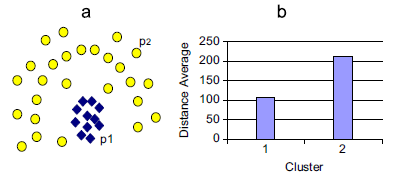
\includegraphics{./Figures/Mitosis_1.png}
		\rule{35em}{0.5pt}
	\caption[Distances between patterns reflect the density structure.]{Distances between patterns reflect the density structure.}
	\label{fig:mitosis_1}
\end{figure}

\subsection{Mitosis Proposed distance relatedness dynamic model}\label{sec:mitosis_proposed}
The dynamic model proposed in \textit{Mitosis} aims at maintaining the consistency of distances between patterns in each cluster.It defines a
distance-relatedness clustering criterion based on the following:
\begin{itemize}
\item A dynamic range neighborhood that depends on the density context of the pattern.
\item Measures that reflect the distance structure of the data.
\end{itemize}

Mitosis distance relatedness model combines both local and global distance relatedness. 
It attempts to cluster the data starting from local measures and extending that to global ones in the course of the algorithm. 
Let the symbols $x$, $y$, $p$, and $q$ denote a pattern, $d(x,y)$ denotes the distance between patterns $x$ and $y$, $a$ denotes the association between two patterns $x$ and $y$, which is the tuple $(x,y,d(x,y))$, $A$ denotes a set of associations, $f$ and $k$ denote user parameters, and $\mu$ denotes the average value of distances.

\textbf{Local distance relatedness}: Any cluster is initially formed from singleton patterns that are related with respect to their neighborhood
average distance measure, and have an in-between distance related to this measure as well. This local merging criterion is a modification of Zahn's inconsistency model.
The rules proposed here are as follows, considering that an average local distance measure is the average of distances in a neighborhood of a pattern as given later
\begin{itemize}
\item The distance between two patterns is related to each of the patterns' average local distance measure, by a factor k.
\item The two patterns' average local distance measures are related by factor k.
\end{itemize}

Figure ~\ref{fig:mitosis_2} illustrates the importance of the mutual consistency between the three entities associated with the local relatedness
criterion; two patterns and a in-between distance. It shows two examples, the first example ($p_1, p_2, d_1$) has two patterns with distance $d_1$related to each patterns' neighborhood distances, yet the two neighborhood distance averages are not related. The second case ($p_3, p_4, d_2$)gives an example of two related neighborhood distance averages, but an unrelated in-between distance $d_2$. The two patterns do not merge in any of these cases, justifying the above proposed local criterion that imposes the mutual consistency between the two neighborhoods and the in between distance. 
The same rationale is used when merging two clusters, but this time considering the clusters' global characteristics.

\begin{figure}[htbp]
	\centering
		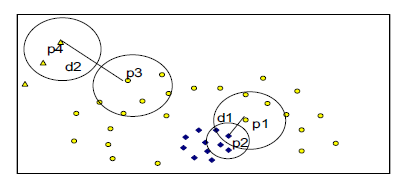
\includegraphics{./Figures/Mitosis_2.png}
		\rule{35em}{0.5pt}
	\caption[Effect of distance inconsistency on merging of patterns]{Effect of distance inconsistency on merging of patterns}
	\label{fig:mitosis_2}
\end{figure}


\textbf{Global distance relatedness}: The property of distance consistency
extends from local relations between neighborhood patterns to global relations between neighboring clusters. The global distance relatedness model follows the same rules of the local relatedness, but with replacing patterns with clusters, a pattern's local average distance with a cluster's average distance, and the distance between two singleton patterns with the distance between the two patterns in the two neighboring clusters. A cluster's average distance(only distances approved to be consistent to the cluster)is used to reflect the distance behavior inside the cluster.

\subsubsection{Distance consistency definitions}
The rules governing consistency of one distance to another cluster's/pattern's average distance, or two clusters'/patterns' average
distance to each other are as follows. given an input parameter $k > 1$:
\begin{itemize}
\item A distance $d(x,y)$ is \textit{k-consistent} to an average $\mu$ of distances if
$d(x, y)<k. \mu$
\item Two distance averages $\mu_1$ and $\mu_2$ are \textit{k-consistent} to each other if $\mu_1 < k.\mu_2 \wedge \mu_2 <k.\mu_1$ or equivalently min$(\mu_1, \mu_2)< k.max(\mu_1, \mu_2)$
\item A distance $d(x,y)$ is \textit{k-consistent} to two averages if $d(x, y)< k.\mu_1 \wedge d(x, y)< k.\mu_2$  i.e. $d(x, y)< k.min(\mu_1, \mu_2)$
\end{itemize}
According to the above definitions the merge criteria are proposed.

\subsubsection{Algorithm's phases}\label{sec:phases}

The algorithm takes as an input the dataset $P$, and 2 main parameters $f$ and $k$. The main steps are as follows:
\begin{itemize}

\item {Get associations:
\begin{itemize}
	\item For each pattern get its dynamic range nearest neighbors using parameter $f$, and calculate local average distance.
	\item Order the associations—ascendingly on distances-between patterns inalist L.
\end{itemize}
}


\item {Merge patterns in to clusters: For each association in L (visited in order), if the merging criterion is satisfied— according to k-, merge
associated patterns/clusters, and update the clusters'measures.}
\item {Refine clusters:
\begin{itemize}
\item For each cluster, add any internal association consistent to the cluster's average.
\item For each cluster, calculate the Harmonic average of distances, and remove associations not consistent to this measure.
\end{itemize}
}
\end{itemize}


\subsection{Implementation Details}\label{sec:implementation}
The class diagram of the implementation of Mitosis is illustrated in figure ~\ref{fig:mitosis_6} where class \textit{Pattern} is an abstract class represents the object to be clustered, in our work the class \textit{Document} implements it, this class stores the representation of the document which is an N-dimentional feature vector each pattern has a reference to its cluster.
The \textit{Association} class contains the relations between the pattern \textit{p} and all other patterns within its dynamic range. Each \textit{Cluster} object contains a list of all patterns and associations consisting it, the \textit{Cluster} object contains the mean value of distances of associations in the cluster $\mu$, and keep updating it while more associations is added to it.

\begin{figure}[htbp]
	\centering
		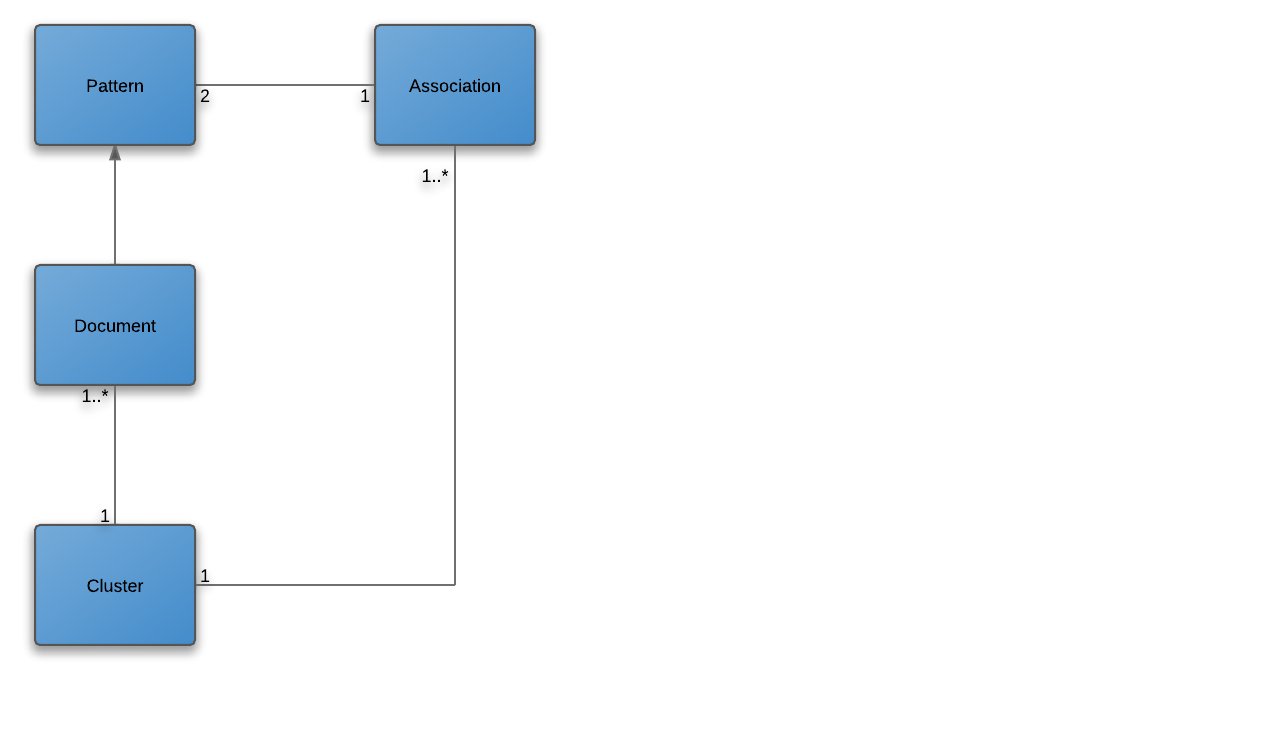
\includegraphics{./Figures/Mitosis_6.png}
		\rule{25em}{0.3pt}
	\caption[Mitosis class Diagram]{Mitosis class Diagram}
	\label{fig:mitosis_6}
\end{figure}

\subsubsection{Loading associations} 
Mitosis requires loading the associations of each pattern which have distance less than $f.min{dist}$ where $f$ is mitosis factor and $min_{dist}$ is the minimum distance betweeen the pattern and all its neighbours.

Given a databse that stores all the distances between all pairs of patterns, loading associations that are in dynamic range for a given pattern $p$ is performed on two steps, first the database is queried to obtain the the instead pattern to $p$ which is at distance $min{dist}$, then the pattern's threshold is calculated as $threshold_{dist} = f \dot dist_{min}$ the database is queried again to obtain all the association with distance less than or equal to $threshold{dist}$.

The clustering algorithm is first applied on two different sets of 2D points (the data set could be found at \citep{Mitosis_2}) for verifying the correctness of the implementation, the results are illustrated in figures ~\ref{fig:mitosis_7} and ~\ref{fig:mitosis_8}.
\begin{figure}[htbp]
	\centering
		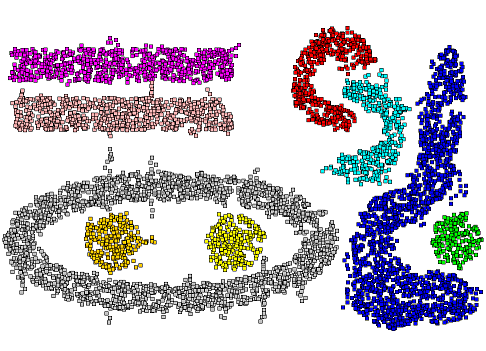
\includegraphics{./Figures/Mitosis_7.png}
		\rule{25em}{0.3pt}
	\caption[Mitosis result on 2D points]{Mitosis result on 2D points}
	\label{fig:mitosis_7}
\end{figure}

\begin{figure}[htbp]
	\centering
		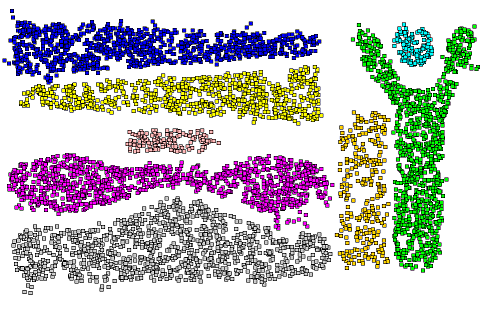
\includegraphics{./Figures/Mitosis_8.png}
		\rule{25em}{0.3pt}
	\caption[Mitosis result on 2D points]{Mitosis result on 2D points}
	\label{fig:mitosis_8}
\end{figure}

Merging phase is a transitive operation, so equivalence classes must be implemented efficiently to avoid any perofrmance bottleneck.
This can be achieved by using \textit{Disjoint sets data structures}
\subsubsection{Disjoint set}

A disjoint-set is a collection $C={S_1, S_2,..., S_k}$ of distinct dynamic sets.
Each set is identified by a member of the set, called representative.
Disjoint set operations:
\begin{itemize}
\item MAKE-SET(x): create a new set with only x. assume x is not already in some other set.
\item UNION(x,y): combine the two sets containing x and y into one new set. A new representative is selected.
\item FIND-SET(x): return the representative of the set containing x.
\end{itemize}
Obviously the \textit{MAKE-SET(x)} operation can be used at the beginning of the algorithm as each pattern will be in a cluster, and the \textit{UNION(x,y)} will be used to marge two clusters.
Next sub-sections will illustrate different implementations
\paragraph{Linked-List Implementation}
Each set as a linked-list, with head and tail, and each node contains value, next node pointer and back-to-representative pointer.
Figure ~\ref{fig:mitosis_3} ~\ref{fig:mitosis_4} shows the operations of the disgoint set.
\begin{itemize}
\item MAKE-SET costs \BigO{1}: just create a single element list.
\item FIND-SET costs \BigO{1}: just return back-to-representative pointer.
\item {UNION(x,y) 
\begin{itemize}
\item {A simple implementation: just appends x to the end of y, updates all back-to-representative pointers in x to the head of y.
Each UNION takes time linear in the x’s length}
\item {Instead appending x to y, appending the shorter list to the longer list.
Associated a length with each list, which indicates how many elements in the list.
}
\end{itemize}
}
\end{itemize}

\begin{figure}[ht]
\begin{minipage}[b]{0.5\linewidth}
\centering
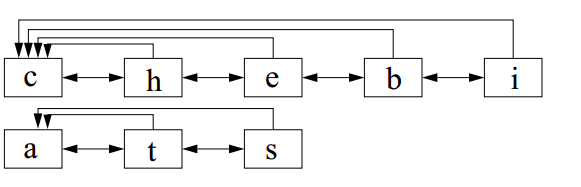
\includegraphics[width=\textwidth]{./Figures/Mitosis_3.png}
\caption{Two sets}
\label{fig:mitosis_3}
\end{minipage}
\hspace{0.5cm}
\begin{minipage}[b]{0.5\linewidth}
\centering
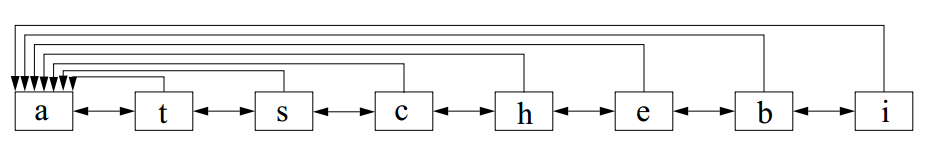
\includegraphics[width=\textwidth]{./Figures/Mitosis_4.png}
\caption{Union of two sets}
\label{fig:mitosis_4}
\end{minipage}
\end{figure}

\paragraph{Disjoint-set Implementation: Forests}
Rooted trees, each tree is a set, root is the representative. Each node points to its parent. Root points to itself.

Three operations
\begin{itemize}
\item MAKE-SET(x): create a tree containing x.  \BigO{1}
\item FIND-SET(x): follow the chain of parent pointers until to the root. \BigO{height of x’s tree}
\item UNION(x,y): let the root of one tree point to the root of the other.  \BigO{1}
\end{itemize}

\textbf{Union by Rank and  Path Compression}
\textit{Union by Rank}: Each node is associated with a rank, which is the upper bound on the height of the node (i.e., the height of subtree rooted at the node), then when UNION, let the root with smaller rank point to the root with larger rank. 
\textit{Path Compression}: used in FIND-SET(x) operation, make each node in the path from x to the root  directly point to the root. Thus reduce the tree height.

\begin{figure}[htbp]
	\centering
		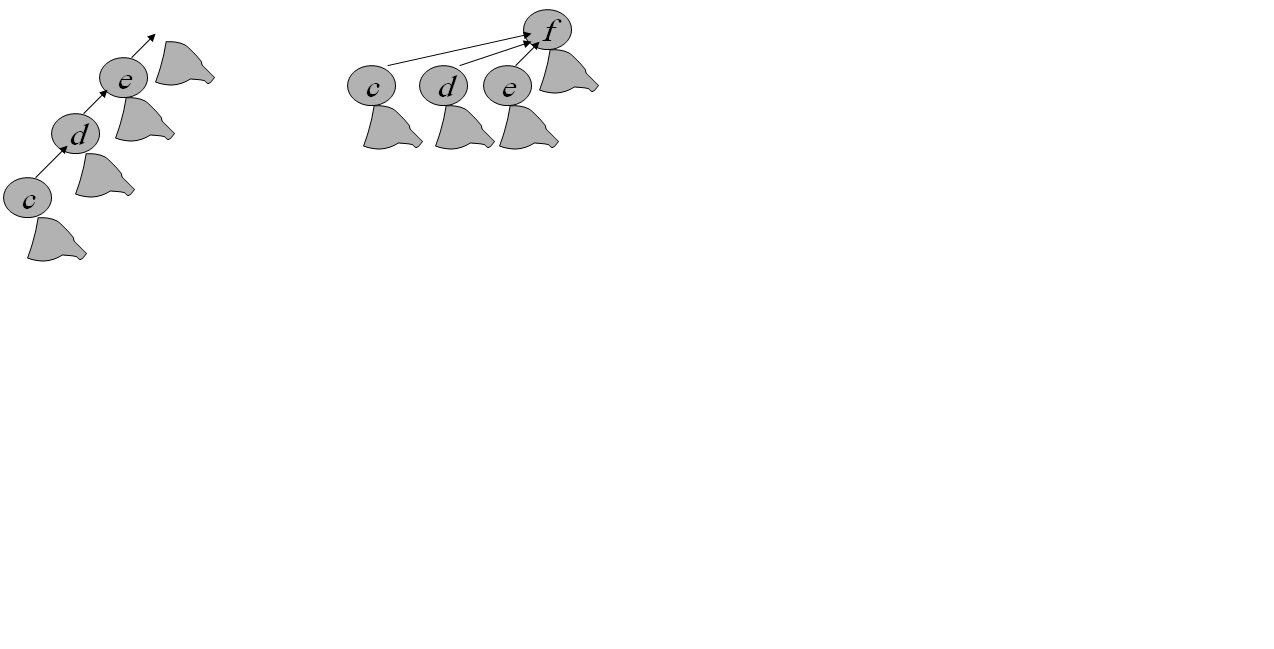
\includegraphics{./Figures/Mitosis_5.png}
		\rule{25em}{0.3pt}
	\caption[Path compression]{Path compression}
	\label{fig:mitosis_5}
\end{figure}
%----------------------------------------------------------------------------------------

 
Chapter 6

\chapter{Tools} % Main chapter title

\label{Chapter6} % For referencing the chapter elsewhere, use \ref{Chapter1} 

\lhead{Chapter 6. \emph{Tools}} % This is for the header on each page - perhaps a shortened title

%----------------------------------------------------------------------------------------

\section{AWN}
Arabic WordNet is the Arabic analogue to the widely used WordNet for the English language. The Arabic WordNet (AWN) is a lexical database of the Arabic language following the development process of Princeton English WordNet and Euro WordNet. It utilizes the Suggested Upper Merged Ontology as an interlingua to link Arabic WordNet to previously developed wordnets. Christiane Fellbaum at Princeton was the project lead. The project was sponsored by DOI/REFLEX.\\
From http://www.globalwordnet.org/AWN/DataSpec.html you can get the XML data exchange specifications of the database. AWN contains about 11,000 synsets (including 1,000 NE).\\

There are several different ways for accessing the database:\\
\begin{itemize}
\item[1] The browser package (available at http://sourceforge.net/projects/awnbrowser/) includes the AWN data and Princeton WN2.0 mappings in a relational database. You can use the export facilities to export the data as XML or CSV to taylor them to your needs .\\
\item[2] The database can also be downloaded in XML format (linked to Princeton WN 2.0) from \url {http://nlp.lsi.upc.edu/awn/get_bd.php}\\
\item[3] A set of basic python functions for accessing the database can be obtained from: \url {http://nlp.lsi.upc.edu/awn/AWNDatabaseManagement.py.gz}\\
\end{itemize}
Functionality:\\
\begin{itemize}
\item AWN Browser: Browsing the database\\
\item AWN can be downloaded in XML format and access its content be directly used at developers' will.\\
\end{itemize}
Technology:\\
    Java, Perl, MySQL\\
Innovation:\\
	One of the most important lexical resources for Arabic language.\\


%-----------------------------------------------------------------------------------------

\section{Crawlers}
we used Web-Harvest for web pages crawling and retrieving the desired data.It’s an Open Source Web Data Extraction tool written in Java. It offers a way to collect desired Web pages and extract useful data from them. In order to do that, it leverages well established techniques and technologies for text/xml manipulation such as XSLT, XQuery and Regular Expressions. Web-Harvest mainly focuses on HTML/XML based web sites which still make vast majority of the Web content. On the other hand, it could be easily supplemented by custom Java libraries in order to augment its extraction capabilities.
Process of extracting data from Web pages is also referred as Web Scraping or Web Data Mining. World Wide Web, as the largest database, often contains various data that we would like to consume for our needs. The problem is that this data is in most cases mixed together with formatting code - that way making human-friendly, but not machine-friendly content. Doing manual copy-paste is error prone, tedious and sometimes even impossible. Web software designers usually discuss how to make clean separation between content and style, using various frameworks and design patterns in order to achieve that. Anyway, some kind of merge occurs usually at the server side, so that the bunch of HTML is delivered to the web client.
Web-Harvest is distributed under BSD License. It gives the freedom for anyone to use, explore, modify, and distribute Web-Harvest, but without any warranty. 
\subsection{Basic concept}
The main goal behind Web-Harvest is to empower the usage of already existing extraction technologies. Its purpose is not to propose a new method, but to provide a way to easily use and combine the existing ones. Web-Harvest offers the set of processors for data handling and control flow. Each processor can be regarded as a function - it has zero or more input parameters and gives a result after execution. Processors could be combined in a pipeline, making the chain of execution. For easier manipulation and data reuse Web-Harvest provides variable context where named variables are stored. The following diagram describes one pipeline execution:

\begin{figure}[htbp]
	\centering
		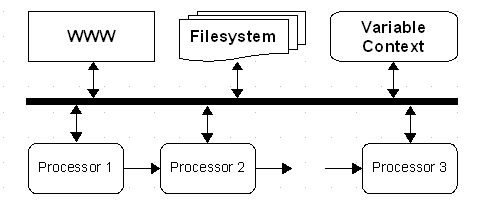
\includegraphics{./Figures/diagram1.png}
		\rule{35em}{0.5pt}
	\caption[Web-Harvest}
\end{figure}


The result of extraction could be available in files created during execution or from the variable context if Web-Harvest is programmatically used.
Configuration language

Every extraction process is defined in one or more configuration files, using simple XML-based language. Each processor is described by specific XML element or structure of XML elements. For the illustration, here is presented an example of configuration file:
you may check the XML configuration file here \ref{crawlersXML}

This configuration contains two pipelines. The first pipeline performs the following steps:
\begin{itemize}
\item [1] HTML content at http://news.bbc.co.uk is downloaded
\item [2] HTML cleaning is performed on downloaded content producing XHTML,
\item [3] XPath expression is searched for, giving URL sequence of page images,
\item [4] New variable named "urlList" is defined containing sequence of image URLs.
\end{itemize}
The second pipeline uses result of the previous execution in order to collect all page images:
\begin{itemize}
\item [1] Loop processor iterates over URL sequence and for every item:
\item [2] Downloads image at current URL,
\item [3] Stores the image on the file system.
\end{itemize}


\section{Corpus}
We used two corpora one of them is Al Jazeera, which contains 4462 article from various categories like Arts,culture,Economy, International, locals, Medical, Society, Sport.
The other corpus is upto-date corpus extracted using crawling tool with predefined XML files from specific News agency Like: Reuters, CNN, BBC, Al Arabiya, Youm7.This corpus was around 160 articles from many categories.



 
%Chapter 7

\chapter{Tools} % Main chapter title

\label{tools} % For referencing the chapter elsewhere, use \ref{Chapter1} 

\lhead{Chapter 7. \emph{Tools}} % This is for the header on each page - perhaps a shortened title

%----------------------------------------------------------------------------------------
This chapter discussed the tools and data sets used, it starts by section ~\ref{pre} which discusses the pre-processing tools used, sections ~\ref{lucene}, ~\ref{awn} and ~\ref{crawlers} demonestrates the usage of \textit{lucene}, \textbf{A}rabic \textbf{W}ord \textbf{N}et (AWN), section ~\ref{corpus} discusses the data sets used, finally section ~\ref{lsa} shows the tools used to implement \textit{LSA}.
\section{Text Preprocessing}\label{pre}
There has been a debate among researchers about the benefits of using morphological tools in Text Analysis. Studies in the \textit{English}
language illustrated that performing stemming during the preprocessing step degrades the performance slightly \citep{pre_8} \citep{pre_9}. 
In this work, the preprocssing consists of three steps: First stop words are removed, second a part of speech tag is assigned to each term and then each term is stemmed.
The output of the preprocessing module is the stem of each term concatenated with its part of speech, to distinguish between noun and verb. for example this sentence "\RL{مجلس الأمن يدرس بياناً يدعو إلى رفع الحصار واقتراح أوروبي}" is mapped to (\RL{مجلس}n, \RL{أمن}n, \RL{يدرس}v, \RL{بيانا}n, \RL{يدعو}v, \RL{رفع}n, \RL{حصار}n, \RL{اقتراح}n, \RL{أوروب}n).

In this work two different techniques are used for stemming: Elkhoja stemmer and Light stemming.

\subsection{Part of speech tagging}

The part of speech tagging is defined as  the process of marking up a word in a text (corpus) as corresponding to a particular part of speech, based on both its definition, as well as its context i.e. relationship with adjacent and related words in a phrase, sentence, or paragraph. 
Stanford Log-linear Part-Of-Speech Tagger \citep{pre_1} \citep{pre_2} is used to tag each term in the document.


\subsection{Stemming}
Stemming is the process of removing all of a word's prefixes and suffixes to produce the stems or the root \citep{pre_3}.
The experiment conducted by \citep{pre_10} indicates that using stemming and dimensionality reduction techniques is not necessary. On the other hand Arabic language is highly derivative where tens or even hundreds of words could be
formed using only one root. The importance of the stemming process comes in the classification and index builders/searchers because it makes the operations fewer dependants on particular form of words, and it reduces the potential size of vocabularies which might otherwise have to contain all possible forms.
Furthermore, a single word may be derived from multiple roots (Attia, 2000). 

Arabic stemming algorithms can be classified, according to the desired level of analysis, as either: 
(a)stem-based or (b)root-based algorithms. Stem-based algorithms, remove prefixes and suffixes from Arabic words, while root-based algorithms reduce stems to roots. After stemming the stem may be further processed to compass the word root in the root-based approach (Darwish, 2003). 
As an example, the stem of “Ketabhom (their book)” is “Ktab (book)” and its root is “Ktb (wrote)” while the stem of the word “Ktateeb
(places for learning Quran)” is the same word “Ktateeb” but the root is  “Ktb (wrote)”.

Early studies performed on IR indicated that using root words is better than using stemmed words as mentioned by (Darwish, 2003). Other studies, by \citep{pre_11} (Moukdad, 2006), reported that the stem-based approach is superior to the root-based approach. An experiment performed by (Darwish et al., 2005) showed that using context to improve the root extraction process may enhance the process of IR slightly compared to the stem-based approach. However, the context root extraction is computationally expensive compared with the stemming. On the contrary, Brants et al. (Brants et al., 2002) reported that performing stemming to the Arabic text increases the ambiguity, and hence using the raw text may be better.



The performance of information retrieval in arabic language is very problematic due to the specific morphological and structural changes in the language: polysemy, irregular and inflected derived forms, various spelling of certain words, various writing of certain combination character, short (diacritics) and long vowels, most of the arabic words contain affixes figures ~\ref{fig:pre_3} ~\ref{fig:pre_4}. To address these problems, several methods have been proposed.
The vocabulary of the arabic language is essentially built from the roots derivation. The roots are words composed of three to five consonants letters. The arabic language has about ten thousand roots, 85\% of them are trilateral. The derivation of words is done by adding affixes (prefix, infix, or suffix) to the root according to several patterns that are around 120 (Al Kharashi, 1999). For example, let us take the root (\RL{كتب}); the words (\RL{كاتب}, \RL{كاتبه},\RL{مكتوب}).
Before applying stemming , the normalization phase is applied before applying these methods, the text normalization takes a character string as input and tries to remove or replace some characters under the predefined rules to converts it into a string of letters (Figure ~\ref{fig:pre_1}).

\begin{figure}[htbp]
	\centering
		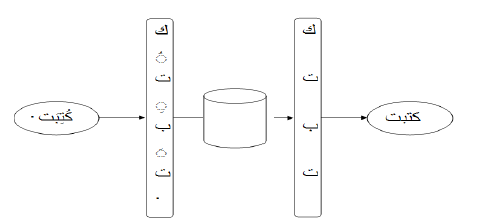
\includegraphics{./Figures/pre_1.png}
		\rule{35em}{0.5pt}
	\caption[Normalization for Arabic text.]{Normalization for Arabic text.}
	\label{fig:pre_1}
\end{figure}

\begin{figure}[htbp]
	\centering
		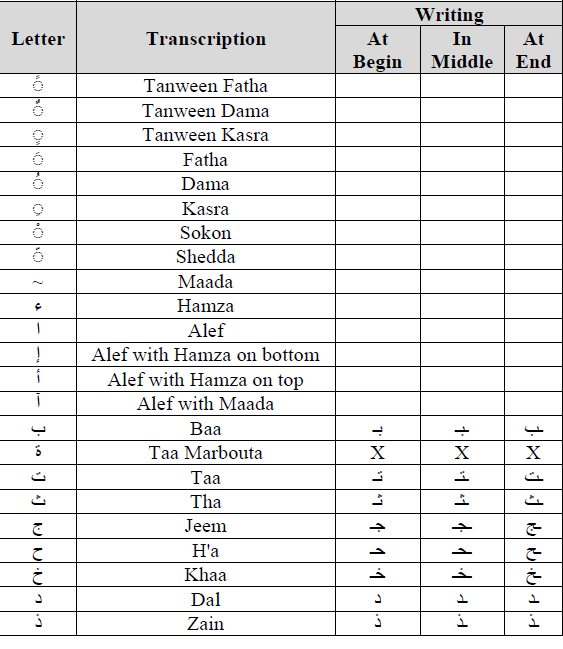
\includegraphics{./Figures/pre_3.png}
		\rule{35em}{0.5pt}
	\caption[Arabic affixes.]{Arabic affixes.}
	\label{fig:pre_3}
\end{figure}

\begin{figure}[htbp]
	\centering
		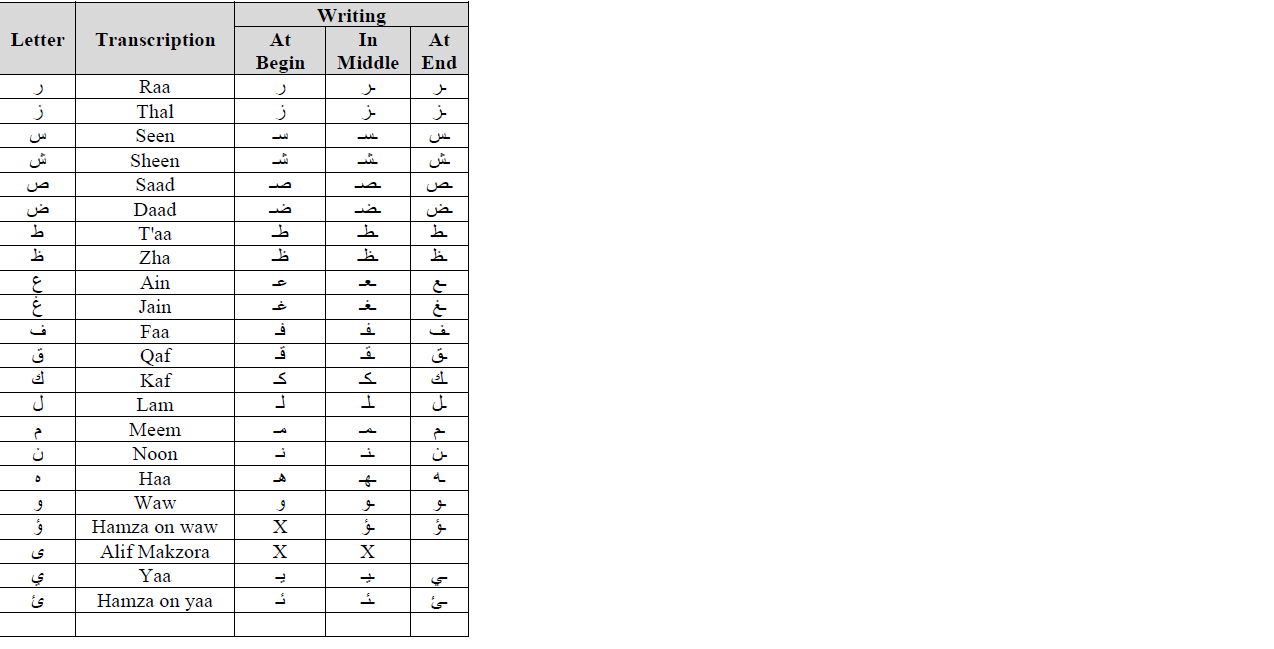
\includegraphics{./Figures/pre_4.png}
		\rule{35em}{0.5pt}
	\caption[Arabic affixes.]{Arabic affixes.}
	\label{fig:pre_4}
\end{figure}

The two components (POS and stemmer) are combined in to one larger component where the document is passed to it and two arrays are returned one contains the part of speech tag while the other stores the stem. The stemming must be perofmed after the POS, because stemming may affect the POS results.

\subsubsection{Stemming based on pattern and affixes}
Arabic patterns are part of the Arabic grammar. They are formed based on the Arabic root \citep{pre_4}. A
root is the base form of a word which can not be further analyzed without the loss of the word's
identity, or it is that part of the word left when all the affixes are removed.
An Arabic root is an ordered sequence of three (\RL{فعل}) or four letters (\RL{فعلل}) from alphabet \citep{pre_5}. The
root has a general, basic meaning which forms the basis of many related meanings. These related
meanings are represented by the root consonants put in different forms called patterns \citep{pre_6}. They
are generated from the process of vocalization and affixation \citep{pre_20}. Table 1 shows a sample of the
Arabic Patterns (Three-Consonant root).
Variations of the root and patterns determine the actual meaning of the word. For example, the
root (\RL{كتب}) with the addition of the letter (\RL{ا}) gives the word (\RL{كتاب}), which means book, while the root pattern combination of 
(\RL{كاتب}) means "one who writes" or "clerk". There are
also some prefixes and suffixes which determine whether a word is a subject marker, pronoun,
preposition, or a definite article. Figure ~\ref{fig:pre_5} and ~\ref{fig:pre_6} illustrates set of derivatives patterns, its corresponding
English word, the position in the language and its Arabic patterns from the Arabic trilateral verbal
root \RL{كتب} (k t b).


\begin{figure}[htbp]
	\begin{center}
		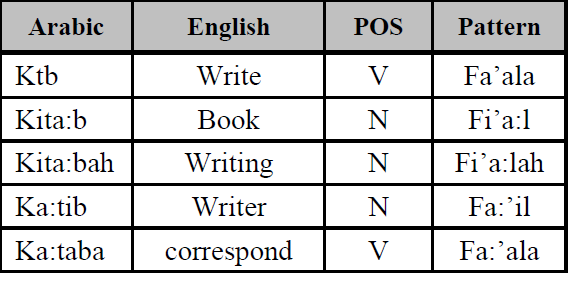
\includegraphics{./Figures/pre_5.png}
		\rule{20em}{0.001pt}
	\end{center}
	\caption[Derivatives of the Arabic trilateral root ‘k t b’.]{Derivatives of the Arabic trilateral root ‘k t b’.}
	\label{fig:pre_5}
\end{figure}

\begin{figure}[htbp]
	\begin{center}
		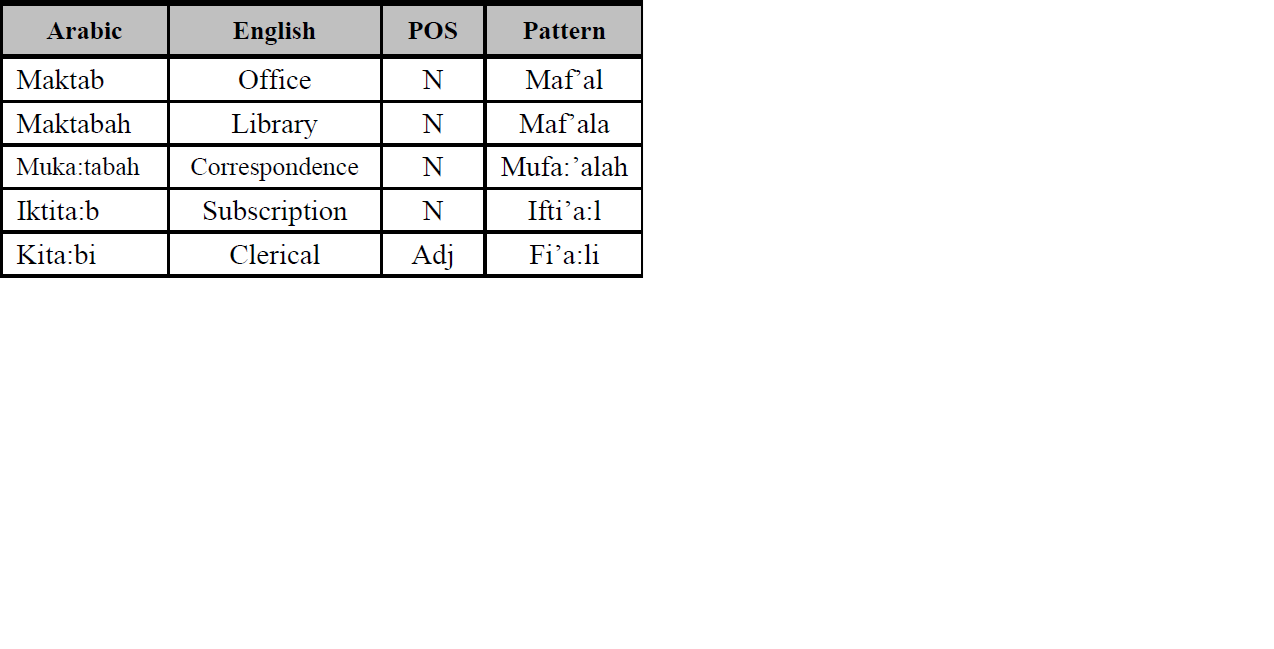
\includegraphics{./Figures/pre_6.png}
		\rule{20em}{0.001pt}
	\end{center}
	\caption[Derivatives of the Arabic trilateral root ‘k t b’.]{Derivatives of the Arabic trilateral root ‘k t b’.}
	\label{fig:pre_6}
\end{figure}


Stemmer based on pattern and affixes Several Stemmer algorithms based on the patterns and affixes have been developed, to find roots with three letters, four and five letters, starting from verbal forms, nouns and adjectives derived from verbs S. Khoja and R. Garside (1999) have proposed a method that involves removing diacritics representing vowelization, the stop words, the punctuation, the numbers, the definite article (\RL{ال}), the inseparable conjunction (\RL{و}), and the longest prefix and suffix. Then, the result is compared to a list of patterns. If a match is found, the characters representing the root in the pattern are extracted.
\subsubsection{Arabic Light Stemmers}
It is not an aggressive practice as the root-based algorithm. The aim of this approach is not to produce the linguistic root of a given Arabic surface form; rather, it is to remove the most frequent suffixes and prefixes.
In Arabic, unlike English, both prefixes and
suffixes are removed for efficient results, but Arabic provides the additional difficulty of infixes
[24]. The difficulty arises because Arabic has two genders, feminine and masculine; three
cardinality, singular, dual, and plural; and three grammatical cases, nominative, genitive, and
accusative. A noun has the nominative case when it is a subject; accusative when it is the object
of a verb; and genitive when it is the object of a preposition. The form of an Arabic noun is
determined by its gender, cardinality, and grammatical case. Light Stemmers remove only prefixes and suffixes. Five pre-defined groups of removable
prefixes and suffixes were offered.

\section{Lucene}\label{lucene}
\label{luceneTool}
Apache Lucene(TM) is a high-performance, full-featured text search engine library written entirely in Java. It is a technology suitable for nearly any application that requires full-text search, especially cross-platform.
\begin{figure}[htbp]
	\begin{center}
		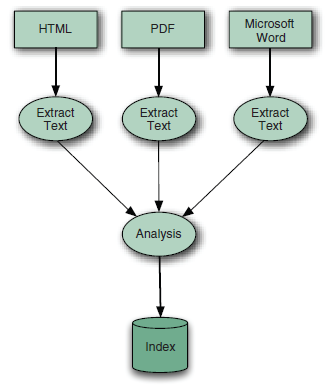
\includegraphics{./Figures/lucene.png}
		\rule{20em}{0.5pt}
	\end{center}
	\caption[Lucene Indexing Process]{Lucene Indexing Process}
	\label{fig:lucene1}
\end{figure}
\begin{figure}[htbp]
	\begin{center}
		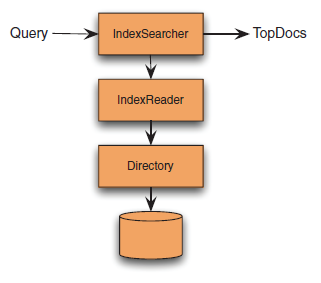
\includegraphics{./Figures/lucene_search.png}
		\rule{20em}{0.5pt}
	\end{center}
	\caption[Lucene searching Process]{Lucene searching Process}
	\label{fig:lucene2}
\end{figure}
Apache Lucene is an open source project available for free download. Please use the links on the right to access Lucene.
Features
Lucene offers powerful features through a simple API:\\
Scalable, High-Performance Indexing
\begin{itemize}
   \item over 95GB/hour on modern hardware
   \item small RAM requirements -- only 1MB heap
  \item  incremental indexing as fast as batch indexing
    \item index size roughly 20-30% the size of text indexed
\end{itemize}
Powerful, Accurate and Efficient Search Algorithms
\begin{itemize}
 \item   ranked searching -- best results returned first
  \item  many powerful query types: phrase queries, wildcard queries, proximity queries, range queries and more
  \item  fielded searching (e.g., title, author, contents)
 \item   date-range searching
   \item sorting by any field
  \item  multiple-index searching with merged results
  \item  allows simultaneous update and searching
\end{itemize}
Cross-Platform Solution
\begin{itemize}
  \item  Available as Open Source software under the Apache License which lets you use Lucene in both commercial and Open Source programs
 \item   100%-pure Java
  \item  Implementations in other programming languages available that are index-compatible
\end{itemize}
\textit{The Apache Software Foundation}\\

The Apache Software Foundation provides support for the Apache community of open-source software projects. The Apache projects are defined by collaborative consensus based processes, an open, pragmatic software license and a desire to create high quality software that leads the way in its field. Apache Lucene, Apache Solr, Apache PyLucene, Apache Open Relevance Project and their respective logos are trademarks of The Apache Software Foundation. All other marks mentioned may be trademarks or registered trademarks of their respective owners.\\
\section{AWN}\label{awn}
Arabic WordNet is the Arabic analogue to the widely used WordNet for the English language. The Arabic WordNet (AWN) is a lexical database of the Arabic language following the development process of Princeton English WordNet and Euro WordNet. It utilizes the Suggested Upper Merged Ontology as an interlingua to link Arabic WordNet to previously developed wordnets. Christiane Fellbaum at Princeton was the project lead. The project was sponsored by DOI/REFLEX.\\
From http://www.globalwordnet.org/AWN/DataSpec.html you can get the XML data exchange specifications of the database. AWN contains about 11,000 synsets (including 1,000 NE).\\

There are several different ways for accessing the database:\\
\begin{itemize}
\item[1] The browser package (available at http://sourceforge.net/projects/awnbrowser/) includes the AWN data and Princeton WN2.0 mappings in a relational database. You can use the export facilities to export the data as XML or CSV to taylor them to your needs .\\
\item[2] The database can also be downloaded in XML format (linked to Princeton WN 2.0) from \url {http://nlp.lsi.upc.edu/awn/get_bd.php}\\
\item[3] A set of basic python functions for accessing the database can be obtained from: \url {http://nlp.lsi.upc.edu/awn/AWNDatabaseManagement.py.gz}\\
\end{itemize}
Functionality:\\
\begin{itemize}
\item AWN Browser: Browsing the database\\
\item AWN can be downloaded in XML format and access its content be directly used at developers' will.\\
\end{itemize}
Technology:\\
    Java, Perl, MySQL\\
Innovation:\\
	One of the most important lexical resources for Arabic language.\\
\begin{figure}[htbp]
	\begin{center}
		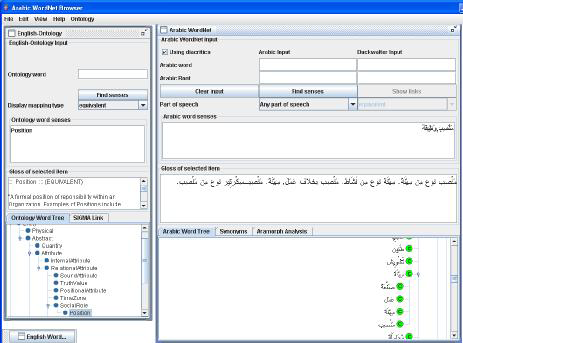
\includegraphics{./Figures/AWNGUI.png}
		\rule{20em}{0.5pt}
	\end{center}
	\caption[AWN GUI]{AWN GUI}
	\label{fig:AWN GUI}
\end{figure}
\begin{figure}[htbp]
	\begin{center}
		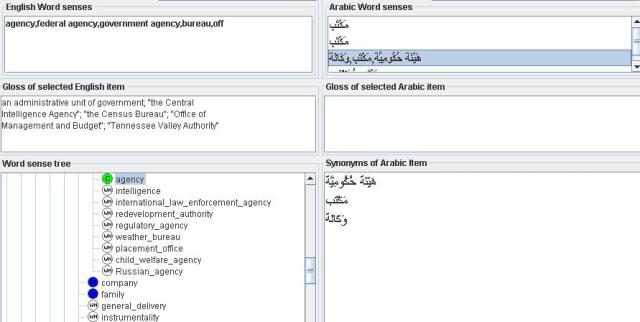
\includegraphics{./Figures/AWNGUI_1.jpg}
		\rule{20em}{0.5pt}
	\end{center}
	\caption[AWN GUI]{AWN GUI}
	\label{fig:AWN GUI}
\end{figure}
%-----------------------------------------------------------------------------------------

\section{Crawlers}\label{crawlers}
we used Web-Harvest for web pages crawling and retrieving the desired data.It’s an Open Source Web Data Extraction tool written in Java. It offers a way to collect desired Web pages and extract useful data from them. In order to do that, it leverages well established techniques and technologies for text/xml manipulation such as XSLT, XQuery and Regular Expressions. Web-Harvest mainly focuses on HTML/XML based web sites which still make vast majority of the Web content. On the other hand, it could be easily supplemented by custom Java libraries in order to augment its extraction capabilities.
Process of extracting data from Web pages is also referred as Web Scraping or Web Data Mining. World Wide Web, as the largest database, often contains various data that we would like to consume for our needs. The problem is that this data is in most cases mixed together with formatting code - that way making human-friendly, but not machine-friendly content. Doing manual copy-paste is error prone, tedious and sometimes even impossible. Web software designers usually discuss how to make clean separation between content and style, using various frameworks and design patterns in order to achieve that. Anyway, some kind of merge occurs usually at the server side, so that the bunch of HTML is delivered to the web client.
Web-Harvest is distributed under BSD License. It gives the freedom for anyone to use, explore, modify, and distribute Web-Harvest, but without any warranty. 
\subsection{Basic concept}
The main goal behind Web-Harvest is to empower the usage of already existing extraction technologies. Its purpose is not to propose a new method, but to provide a way to easily use and combine the existing ones. Web-Harvest offers the set of processors for data handling and control flow. Each processor can be regarded as a function - it has zero or more input parameters and gives a result after execution. Processors could be combined in a pipeline, making the chain of execution. For easier manipulation and data reuse Web-Harvest provides variable context where named variables are stored. The following diagram describes one pipeline execution:

\begin{figure}[htbp]
	\centering
		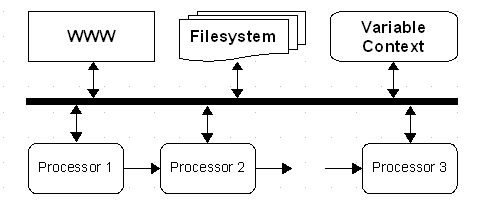
\includegraphics{./Figures/diagram1.png}
		\rule{35em}{0.5pt}
	\caption[Web-Harvest]{Web-Harvest}
\end{figure}


The result of extraction could be available in files created during execution or from the variable context if Web-Harvest is programmatically used.
Configuration language

Every extraction process is defined in one or more configuration files, using simple XML-based language. Each processor is described by specific XML element or structure of XML elements. For the illustration, here is presented an example of configuration file:
you may check the XML configuration file here \ref{crawlersXML}

This configuration contains two pipelines. The first pipeline performs the following steps:
\begin{itemize}
\item [1] HTML content at http://news.bbc.co.uk is downloaded
\item [2] HTML cleaning is performed on downloaded content producing XHTML,
\item [3] XPath expression is searched for, giving URL sequence of page images,
\item [4] New variable named "urlList" is defined containing sequence of image URLs.
\end{itemize}
The second pipeline uses result of the previous execution in order to collect all page images:
\begin{itemize}
\item [1] Loop processor iterates over URL sequence and for every item:
\item [2] Downloads image at current URL,
\item [3] Stores the image on the file system.
\end{itemize}


\section{Corpus}\label{corpus}
We used two corpora one of them is Al Jazeera, which contains 4462 article from various categories like Arts,culture,Economy, International, locals, Medical, Society, Sport.
The other corpus is upto-date corpus extracted using crawling tool with predefined XML files from specific News agency Like: Reuters, CNN, BBC, Al Arabiya, Youm7.This corpus was around 160 articles from many categories.


\section{LSA Tools}\label{lsa}
\subsection{Python}
\subsubsection{Description}
Python is a remarkably powerful dynamic programming language that is used in a wide variety of application domains. Python is often compared to Tcl, Perl, Ruby, Scheme or Java. Some of its key distinguishing features include:
\begin{itemize}
\item very clear, readable syntax
\item strong introspection capabilities
\item intuitive object orientation
\item natural expression of procedural code
\item full modularity, supporting hierarchical packages
\item exception-based error handling
\item very high level dynamic data types
\item extensive standard libraries and third party modules for virtually every task
\item extensions and modules easily written in C, C++ (or Java for Jython, or .NET languages for IronPython)
\item embeddable within applications as a scripting interface
\end{itemize}
\subsubsection{Usage}
Python was used as the main programming language for the LSA implementation due to being extensible till the Ram size and having many third party packages for haonendling SVD calculations
\subsection{DIVISI2}
\subsubsection{Description}
Divisi is a sparse SVD toolkit for Python that is particularly designed for working with semantic networks.
\subsubsection{Usage}
Divisi was used to calculate SVD in a sparse way as the term vs. document matrix is so sparse so sparse SVD is more efficient than normal one
\subsection{PyTables}
\subsubsection{Description}
PyTables is a package for managing hierarchical datasets and designed to efficiently and easily cope with extremely large amounts of data. 
PyTables is built on top of the HDF5 library, using the Python language and the NumPy package. It features an object-oriented interface that, combined with C extensions for the performance-critical parts of the code (generated using Cython), makes it a fast, yet extremely easy to use tool for interactively browse, process and search very large amounts of data. One important feature of PyTables is that it optimizes memory and disk resources so that data takes much less space (specially if on-flight compression is used) than other solutions such as relational or object oriented databases.
\subsubsection{Usage}
PyTables was used to save the term vs. document matrix in a h5 file format which caches part of the array in the Ram so as to be able to deal with array sizes bigger than that of the Ram. Also, the array is saved in a compressed format.
\subsection{Numpy}
\subsubsection{Description}
NumPy is the fundamental package for scientific computing with Python. It contains among other things:
\begin{itemize}
\item a powerful N-dimensional array object
\item sophisticated (broadcasting) functions
\item tools for integrating C/C++ and Fortran code
\item useful linear algebra, Fourier transform, and random number capabilities
\end{itemize}
Besides its obvious scientific uses, NumPy can also be used as an efficient multi-dimensional container of generic data. Arbitrary data-types can be defined. This allows NumPy to seamlessly and speedily integrate with a wide variety of databases.
\subsubsection{Usage}
Numpy was used to perform matrix operations like: calculating the cosine similarity, calculate the vector representation of the document.


 
%Chapter 8

\chapter{System Performance Evaluation} % Main chapter title

\label{eval} % For referencing the chapter elsewhere, use \ref{eval} 

\lhead{System Performance Evaluation. \emph{System Performance Evaluation}} % This is for the header on each page - perhaps a shortened title
%----------------------------------------------------------------------------------------
In this chapter we present our system\'s performance evaluation and performance analysis. However, we need to stress again on the lack of resource for Arabic language and how that caused performance degradation of some components of the system. The chapter is organized as follows; resources are discussed from the performance point-of-view in section ~\ref{sec:challenges}, used performance measures are explained in section ~\ref{sec:tech}, while the design of the test cases is explained in section ~\ref{sec:test}. Finally, the obtained results are viewed in the last section of the chapter section ~\ref{sec:results}.

\section{Challenges}\label{sec:challenges}
This is section we give an overall discussion of the resources for Arabic language and its limitations from the perspective of performance. The main components of our system are Web Crawlers, Pre-processing tools, Similarity measure, Clustering algorithms and Recommender System. \\
We used Web Harvest as our web crawler which surfs some given URL domains and retrieves web pages\' content. Web Harvest has a good performance and a plausible throughput given the number of web pages that were crawled. \\For the Pre-processing part we used Stanford\'s POS which gave a very good performance for Arabic language. We also used different Stemmers, light stemmer like the Arabic stemmer used by Lucene. However, we also used El-Khoga stemmer as different type of stemmer. All the Pre-processing components gave a plausible output and could scale-up to processing thousands of documents.\\ 
For the Similarity part, we examined different approaches; Lexical, Knowledge-based and Corpus-based similarities. For Lexical similarity, we used Lucene to build inverted index on the retrieved documents and calculate the TF-IDF. \\
Lucene is proved to be highly optimized and it gave a very good performance with processing Arabic text. For Knowledge-based approach, first we tried Arabic WordNet (AWN) to model the concepts and the knowledge of the Arabic language. \\
Unfortunately, AWN was a performance bottleneck in our system. The running time of AWN resulted in a significant degradation in the system\'s performance. AWN could not scale-up to handle large data-sets. Wikipedia as ontology was our alternative to AWN. Wikipedia approach was very promising when compared to AWN, but, due to time constraints, we could not investigate this new approach as much as we did with the AWN approach. The Wikipedia approach scaled-up to relatively large data-sets of documents and allowed us to compute hundreds of thousands of documents similarities. Indeed, Wikipedia wasn\'t computationally expensive when compared to AWN. 
Another resource that affected our performance evaluation process was the existence of a labeled training set for Arabic language. Another thing was that, we had to run the web crawlers on News websites as it\'s almost the only on-line content that is written in formal Arabic language. \\

Although Arabic language is used by more than $330$ million Arabic speakers, there are few systems that we can compare our system with, also there are no human-judged dataset for Arabic text. We used Aljazeera data set \footnote[1]{Available online at http://filebox.vt.edu/users/dsaid/AljNews.tar.gz} that is categorized in to $8$ categories to measure the accuracy of the different clustering algorithms.

Due to all the previously explained issues, with the addition of our hardware resources� capabilities and the wide set of alternatives to almost each of the system�s components, we were limited by a few number of experiments. A single run might take more than 12 hours to produce an output. These, previously mentioned, reasons also limited our ability to run the clustering algorithms like Mitosis and DBSCAN with a wide range of parameters� values to be able to tune the algorithms with the best parameter set.\\
However, we were able to test the whole system on two different randomly selected data-sets. The data-set was collected from Aljazeera news website. Some of the system techniques were tested on three different data-sets. We examined, as large as possible, different ranges of parameters for the Mitosis clustering algorithm. We also considered different performance measures like Purity and Confusion Matrix.\\


\section{Evaluation techniques}\label{sec:tech}
We chose to evaluate the performance of the system by evaluating the performance of the clustering algorithms. We tested every component of the system individually before integrating it with the other system components. However, many test runs were conducted to evaluate the overall system, which was achieved by evaluating the clustering algorithm. We also chose Purity and Confusion Matrix as performance measure techniques. In this section we will discuss the performance measurement technique that we used. \\
The cluster hypothesis states the fundamental assumption we make when using clustering in information retrieval,\textit{"Documents in the same cluster behave similarly with respect to relevance to information needs."} The hypothesis states that if there is a document from a cluster that is relevant to a search request, then it is likely that other documents from the same cluster are also relevant. This is because clustering puts together documents that share many terms.\\
Typical objective functions in clustering formalize the goal of attaining high intra-cluster similarity (documents within a cluster are similar) and low inter-cluster similarity (documents from different clusters are dissimilar). This is an internal criterion for the quality of a clustering. But good scores on an internal criterion do not necessarily translate into good effectiveness in an application. An alternative to internal criteria is direct evaluation in the application of interest. For search result clustering, we may want to measure the time it takes users to find an answer with different clustering algorithms. This is the most direct evaluation, but it is expensive, especially if large user studies are necessary.\\
As a surrogate for user judgments, we can use a set of classes in an evaluation benchmark or gold standard. The gold standard is ideally produced by human judges with a good level of inter-judge agreement. We can then compute an external criterion that evaluates how well the clustering matches the gold standard classes.\\

\subsection{Purity}
This section introduces external criterion of clustering quality. Purity is a simple and transparent evaluation measure. To compute Purity, each cluster is assigned to the class which is most frequent in the cluster, and then the accuracy of this assignment is measured by counting the number of correctly assigned documents and dividing by N.
Formally:
\begin{equation}
Purity(\omega,C) =\frac{1}{N}\sum_k max_j|w_k \cap c_j|
\end{equation}
Where $\omega= \{w_1,w_2,�,w_K \}$  is the set of clusters,  $C= \{c_1,c_2,�,c_J \}$ is the set of classes and N is the total number of documents. We interpret $w_k$ as the set of documents in $w_k$ and $c_j$ as the set of documents $inc_j$. We present an example of how to compute purity in Figure ~\ref{fig:purityFig}. Bad clustering has purity values close to 0; a perfect clustering has a purity of 1. High purity is easy to achieve when the number of clusters is large - in particular, purity is 1 if each document gets its own cluster.
\begin{figure}[htbp]
	\centering
		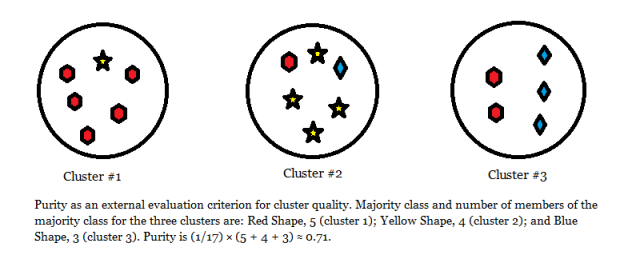
\includegraphics{./Figures/Purityexample.png}
		\rule{35em}{0.5pt}
	\caption[Purity Example]{Purity Example}
	\label{fig:purityFig}
\end{figure}
\subsection{F - Score}
In statistics, the F score (also F-measure) is a measure of a test's accuracy. It considers both the precision $p$ and the recall $r$ of the test to compute the score: $p$ is the number of correct results divided by the number of all returned results and $r$ is the number of correct results divided by the number of results that should have been returned. The F score can be interpreted as a weighted average of the precision and recall, where an F score reaches its best value at 1 and worst score at 0.
The traditional F-measure or balanced F-score (F1 score) is the harmonic mean of precision and recall see equation ~\ref{fmeasure}
\subsection{Confusion Matrix}
An important tool for analyzing the performance of a classifier for $J > 2$ classes is the confusion matrix. The confusion matrix shows for each pair of classes {c1, c2}, how many documents from c1 were incorrectly assigned to c2. It is a specific table layout that allows visualization of the performance of an algorithm. Each column of the matrix represents the instances in a predicted class, while each row represents the instances in an actual class. The name stems from the fact that it makes it easy to see if the system is confusing two classes (i.e. commonly mislabeling one as another). The confusion matrix can help pinpoint opportunities for improving the accuracy of the system. In predictive analytics, a table of confusion (sometimes also called a confusion matrix), is a table with two rows and two columns that reports the number of false positives, false negatives, true positives and true negatives. This allows more detailed analysis. The final table of confusion would contain the average values for all classes combined.

\begin{table}[ht]
\caption{Table of Confusion} % title of Table
\centering  % used for centering table
\begin{tabular}{c c c} % centered columns (5 columns)
\hline\hline                        %inserts double horizontal lines
 & Same Cluster & Different Clusters \\ [0.5ex] % inserts table 
%heading
\hline                  % inserts single horizontal line
Same Class & True Positive (TP)&False Negative (FN)\\ % inserting body of the table
Different Classes & False Positive (FP)& True Negative (TN)  \\[1ex]      % [1ex] adds vertical space
\hline %inserts single line
\end{tabular}
\label{table:conf} % is used to refer this table in the text
\end{table}

From the table of confusion ~\ref{table:conf}, we can calculate Precision, Recall and F-Score as follows:

\begin{equation}
Precision =\frac{TP}{TP + FP}
\end{equation}

\begin{equation}
Recall =\frac{TP}{TP + FN}
\end{equation}

\begin{equation}
\label{fmeasure}
F-Score = 2\times \frac {Recall\times Precision}{Recall + Precision}
\end{equation}

\section{Experiments Design}\label{sec:test}
In this Section we describes how our experiments were performed, what parameters we changed and what variations of modules we used.
Our Experiment is divided to three main variations which are: Lexical-Based Similarity, Semantic Wiki-based Similarity and finally LSA-based Similarity. In each case we compute the $N\times N$ similarities between the documents of the three datasets used.\\
Next we feed these results to our Clustering module based on Mitosis Clustering Technique, where this algorithm takes two parameters as input $(f,k)$ you may refer to section ~\ref{mitosis} for further information.
Finally we try to Cluster the input documents according to the input similarity measure and with various ranges for the Mitosis paramters$(f,k)$, to get the parameters where maximum results are given.

\section{Results and discussion}\label{sec:results}
This section is dedicated for displaying our experiments results, parameter tuning for mitosis and doing some analysis on these results.you can find tables next in this chapter showing the experimental results we have got, where each similarity technique has 2 tables, one for Purity values and the other for F-Score values. This experiment is repeated 2 times for different datasets. you can find these results in tables ~\ref{tables}.\\

Also we used the mean of the obtained purity values to get an overall performace evaluation across various ranges of Mitosis paramters as illustrated in Figures ~\ref{fig:F10}, ~\ref{fig:F11}, ~\ref{fig:F16} \& ~\ref{fig:F30}.\\
Next we provide a simple comparison in Figures ~\ref{fig:F120} \& ~\ref{fig:F121} using the maximum purity measure obtained and Figures  ~\ref{fig:F50} \& ~\ref{fig:F15} using also the maximum obtained F-Score values.

\section{Experimental Results}
\label{tables}
\begin{figure}[htbp]
	\centering
		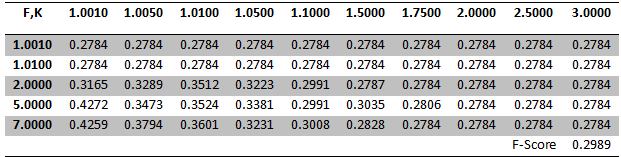
\includegraphics{./Figures/lexical_F_DS1.png}
		\rule{35em}{0.5pt}
	\caption[F-Measure for Lexical Similarity on Dataset one]{F-Measure for Lexical Similarity on Dataset one}
	\label{fig:purity1}
\end{figure}

\begin{figure}[htbp]
	\centering
		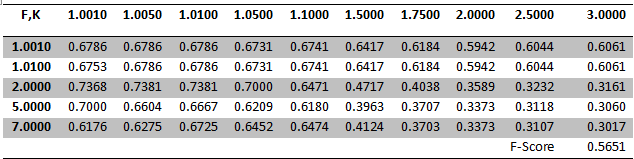
\includegraphics{./Figures/lexical_F_DS2.png}
		\rule{35em}{0.5pt}
	\caption[F-Measure for Lexical Similarity on Dataset Two]{F-Measure for Lexical Similarity on Dataset Two}
	\label{fig:purity2}
\end{figure}

\begin{figure}[htbp]
	\centering
		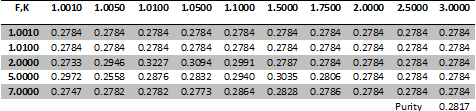
\includegraphics{./Figures/lexical_Purity_DS1.png}
		\rule{35em}{0.5pt}
	\caption[Purity for Lexical Similarity on Dataset one]{Purity for Lexical Similarity on Dataset one}
	\label{fig:purity3}
\end{figure}

\begin{figure}[htbp]
	\centering
		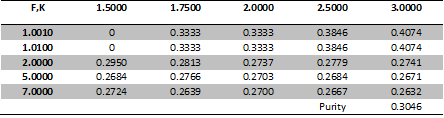
\includegraphics{./Figures/lexical_Purity_DS2.png}
		\rule{35em}{0.5pt}
	\caption[Purity for Lexical Similarity on Dataset two]{Purity for Lexical Similarity on Dataset two}
	\label{fig:purity4}
\end{figure}

\begin{figure}[htbp]
	\centering
		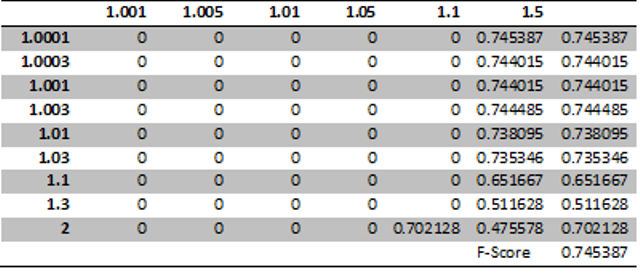
\includegraphics{./Figures/lsa_F_DS1.png}
		\rule{35em}{0.5pt}
	\caption[F-Measure for LSA Similarity on Dataset one]{F-Measure for LSA Similarity on Dataset one}
	\label{fig:F1}
\end{figure}

\begin{figure}[htbp]
	\centering
		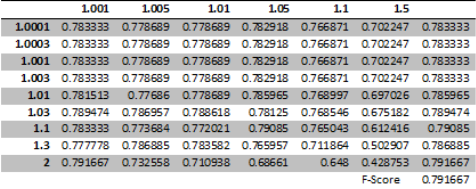
\includegraphics{./Figures/lsa_F_DS2.png}
		\rule{35em}{0.5pt}
	\caption[F-Measure for LSA Similarity on Dataset Two]{F-Measure for LSA Similarity on Dataset Two}
	\label{fig:F2}
\end{figure}

\begin{figure}[htbp]
	\centering
		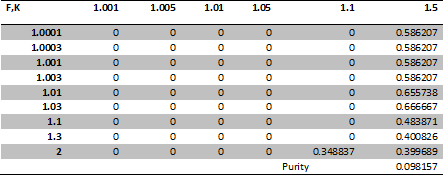
\includegraphics{./Figures/lsa_Purity_DS1.png}
		\rule{35em}{0.5pt}
	\caption[Purity for LSA Similarity on Dataset one]{Purity for LSA Similarity on Dataset one}
	\label{fig:F3}
\end{figure}

\begin{figure}[htbp]
	\centering
		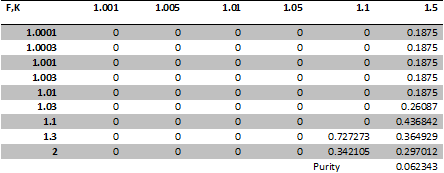
\includegraphics{./Figures/lsa_Purity_DS2.png}
		\rule{35em}{0.5pt}
	\caption[Purity for LSA Similarity on Dataset Two]{Purity for LSA Similarity on Dataset Two}
	\label{fig:F4}
\end{figure}

\begin{figure}[htbp]
	\centering
		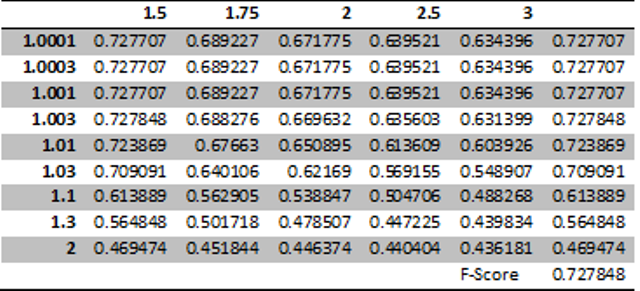
\includegraphics{./Figures/wiki_F_DS1.png}
		\rule{35em}{0.5pt}
	\caption[F-Measure for Wikipedia Similarity on Dataset one]{F-Measure for Wikipedia Similarity on Dataset one}
	\label{fig:F5}
\end{figure}

\begin{figure}[htbp]
	\centering
		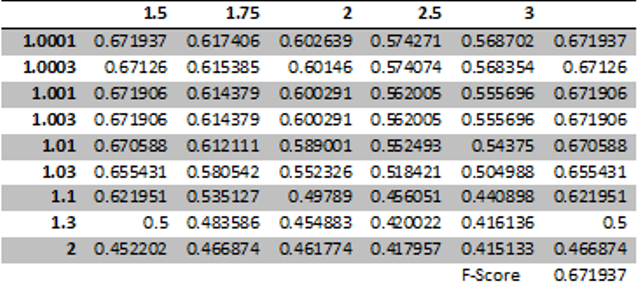
\includegraphics{./Figures/wiki_F_DS2.png}
		\rule{35em}{0.5pt}
	\caption[F-Measure for Wikipedia Similarity on Dataset Two]{F-Measure for Wikipedia Similarity on Dataset Two}
	\label{fig:F6}
\end{figure}

\begin{figure}[htbp]
	\centering
		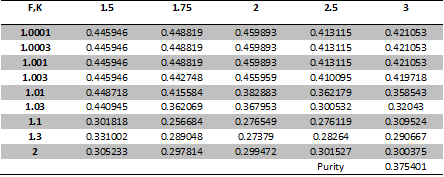
\includegraphics{./Figures/wiki_Purity_DS1.png}
		\rule{35em}{0.5pt}
	\caption[Purity for Wikipedia Similarity on Dataset one]{Purity for Wikipedia Similarity on Dataset one}
	\label{fig:F7}
\end{figure}

\begin{figure}[htbp]
	\centering
		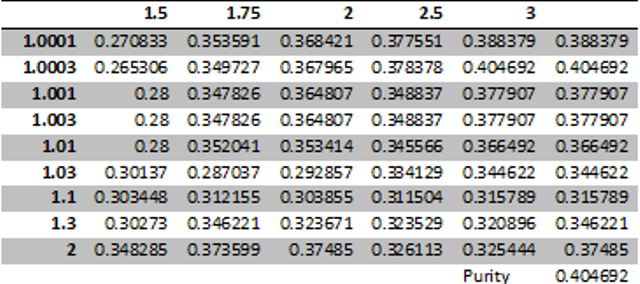
\includegraphics{./Figures/wiki_Purity_DS2.png}
		\rule{35em}{0.5pt}
	\caption[Purity for Wikipedia Similarity on Dataset one]{Purity for Wikipedia Similarity on Dataset Two}
	\label{fig:F8}
\end{figure}
%==================================MEAN=========================================
\begin{figure}[htbp]
	\centering
		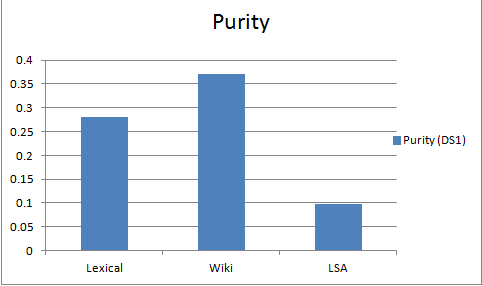
\includegraphics{./Figures/Purity_DS1.png}
		\rule{35em}{0.5pt}
	\caption[Comparison between Purity Values of Different Techniques of Similarity on Dataset one]{Comparison between Purity Values of Different Techniques of Similarity on Dataset one}
	\label{fig:F10}
\end{figure}
\begin{figure}[htbp]
	\centering
		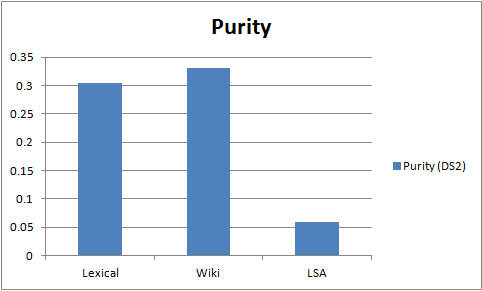
\includegraphics{./Figures/Purity_DS2.png}
		\rule{35em}{0.5pt}
	\caption[Comparison between Purity Values of Different Techniques of Similarity on Dataset Two]{Comparison between Purity Values of Different Techniques of Similarity on Dataset Two}
	\label{fig:F11}
\end{figure}


\begin{figure}[htbp]
	\centering
		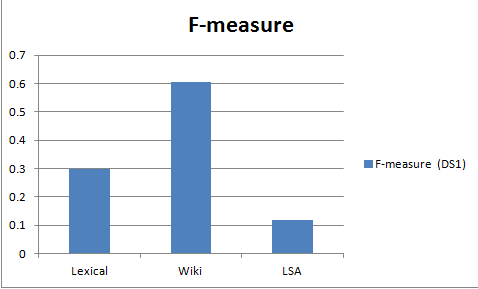
\includegraphics{./Figures/F_DS1.png}
		\rule{35em}{0.5pt}
	\caption[Comparison between Purity Values of Different Techniques of Similarity on Dataset one]{Comparison between Purity Values of Different Techniques of Similarity on Dataset one}
	\label{fig:F16}
\end{figure}
\begin{figure}[htbp]
	\centering
		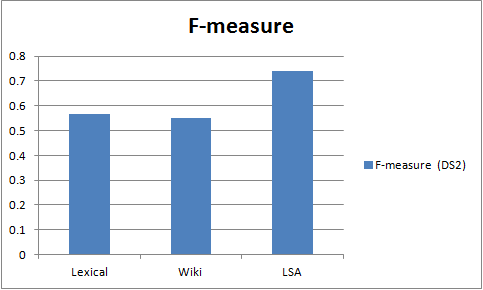
\includegraphics{./Figures/F_DS2.png}
		\rule{35em}{0.5pt}
	\caption[Comparison between Purity Values of Different Techniques of Similarity on Dataset Two]{Comparison between Purity Values of Different Techniques of Similarity on Dataset Two}
	\label{fig:F30}
\end{figure}

%============================MAX==============================
\begin{figure}[htbp]
	\centering
		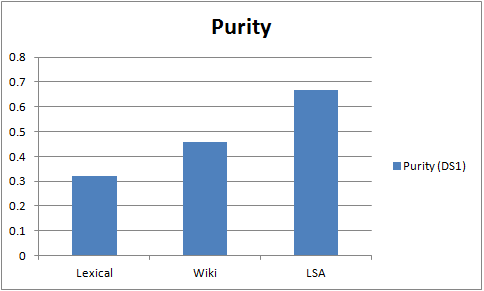
\includegraphics{./Figures/Purity_DS1_1.png}
		\rule{35em}{0.5pt}
	\caption[Comparison between Purity Values of Different Techniques of Similarity on Dataset one]{Comparison between Purity Values of Different Techniques of Similarity on Dataset one}
	\label{fig:F120}
\end{figure}

\begin{figure}[htbp]
	\centering
		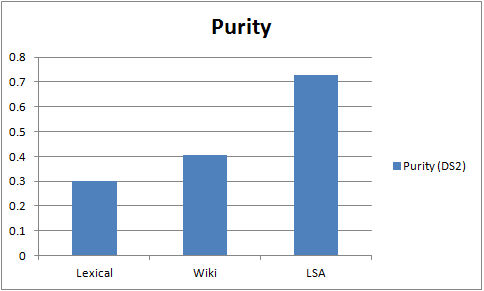
\includegraphics{./Figures/Purity_DS2_1.png}
		\rule{35em}{0.5pt}
	\caption[Comparison between Purity Values of Different Techniques of Similarity on Dataset Two]{Comparison between Purity Values of Different Techniques of Similarity on Dataset Two}
	\label{fig:F121}
\end{figure}
\clearpage
\begin{figure}[htbp]
	\centering
		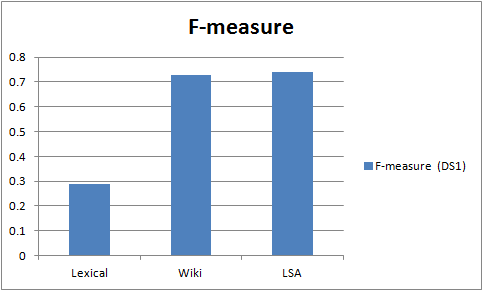
\includegraphics{./Figures/F_DS1_1.png}
		\rule{35em}{0.5pt}
	\caption[Comparison between Purity Values of Different Techniques of Similarity on Dataset one]{Comparison between Purity Values of Different Techniques of Similarity on Dataset one}
	\label{fig:F50}
\end{figure}

\begin{figure}[htbp]
	\centering
		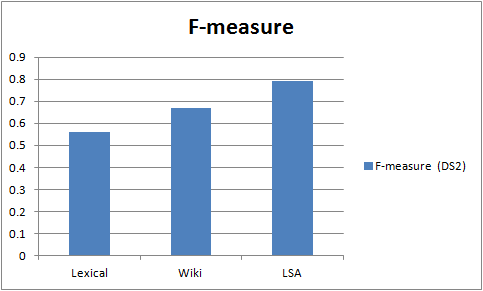
\includegraphics{./Figures/F_DS2_1.png}
		\rule{35em}{0.5pt}
	\caption[Comparison between Purity Values of Different Techniques of Similarity on Dataset Two]{Comparison between Purity Values of Different Techniques of Similarity on Dataset Two}
	\label{fig:F15}
\end{figure}

 
%Chapter 9

\chapter{Conclusion and future work} % Main chapter title

\label{future} % For referencing the chapter elsewhere, use \ref{future} 

\lhead{Conclusion and future work. \emph{Conclusion and future work}} % This is for the header on each page - perhaps a shortened title
%----------------------------------------------------------------------------------------

\section{Future work}
\subsection{Enhancing the semantic similarity module}
\subsubsection{Spreading activity}
Adding Spreading activity in wikipedia similarity module.
Spreading Activation is a technique that has been widely
adopted for associative retrieval (Crestani 1997). In associative
retrieval the idea is that it is possible to retrieve
relevant documents if they are associated with other
documents that have been considered relevant by the user.
In Wikipedia the links between articles show association
between concepts of articles and hence can be used as such
for finding related concepts to a given concept. The algorithm
starts with a set of activated nodes and in each iteration
the activation of nodes is spread to associated nodes.
The spread of activation may be directed by addition of
different constraints like distance constraints, fan out constraints,
path constraints, threshold etc. These parameters
are mostly domain specific.

\subsubsection{Probabilistic Latent Analysis (PLSA)}
PLSA models the probability of each co-occurrence as a mixture of conditionally independent multinomial distributions:
\begin{equation}
P(w,d) = \sum_{c} P(c)P(d|c)P(w|c)= P(d)\sum_{c}P(c|d)P(w|c)
\end{equation}
The first formulation is the symmetric formulation, where $w$ and $d$ are both generated from the latent class $c$ in similar ways (using the conditional probabilities $P(d|c)$ and $P(w|c)$), whereas the second formulation is the asymmetric formulation, where, for each document $d$, a latent class is chosen conditionally to the document according to $P(c|d)$, and a word is then generated from that class according to $P(w|c)$. Although we have used words and documents in this example, the co-occurrence of any couple of discrete variables may be modelled in exactly the same way.
So, the number of parameters is equal to . The number of parameters grows linearly with the number of documents. In addition, although PLSA is a generative model of the documents in the collection it is estimated on, it is not a generative model of new documents.

Other enhancements can be obtained by giving name entities(NER), titles, first statements of the article higher weight in the similarity.\newline
Or by using the database of Arabic wordNet(not the whole the project), as the existing modules that load from database have poor performance.

\subsection{Recommendation system}
\subsubsection{Na�ve Bayes Profile Model}
The model estimates the a posteriori probability, $P (c|d)$, of document $d$ belonging to class $c$. This estimation is based on the a priori probability, $P(c)$, the probability of observing a document in class $c$, $P (d|c)$, the probability of observing the document $d$ given $c$ and, $P (d)$, the probability of observing the instance $d$. Using these probabilities, the Bayes theorem is applied to calculate $P (c|d)$ as follows:
\begin{equation}
P(c|d) = \frac{P(c)P(d|c)}{P(d)}
\end{equation}
\subsection{System evaluation}
Evaluating more combinations of the used modules (Elkhoja stemmer, DBSCAN for clustering, wikipedia similarity module with feature reduction technique PCA)
\begin{itemize}
\item Using different clustering algorithms (CHAMELEON, hierarchical clustering).
\item Integrating the recommendation system with the social network.
\item Adding incremental clustering.
\end{itemize}
 

%----------------------------------------------------------------------------------------
%	THESIS CONTENT - APPENDICES
%----------------------------------------------------------------------------------------

\addtocontents{toc}{\vspace{2em}} % Add a gap in the Contents, for aesthetics

\appendix % Cue to tell LaTeX that the following 'chapters' are Appendices

% Include the appendices of the thesis as separate files from the Appendices folder
% Uncomment the lines as you write the Appendices

% Appendix A

\chapter{Appendix Title Here} % Main appendix title

\label{AppendixA} % For referencing this appendix elsewhere, use \ref{AppendixA}

\lhead{Appendix A. \emph{Appendix Title Here}} % This is for the header on each page - perhaps a shortened title

\section{JIGSAW Disambiguation}
\begin{algorithmic}
\If {$i\geq maxval$}
    \State $i\gets 0$
\Else
    \If {$i+k\leq maxval$}
        \State $i\gets i+k$
    \EndIf
\EndIf
\end{algorithmic}

% Appendix B

\chapter{Used algorithms Pseudocode} % Main appendix title

\label{AppendixB} % For referencing this appendix elsewhere, use \ref{AppendixA}

\lhead{Used algorithms Pseudocode\emph{Used algorithms Pseudocode}} % This is for the header on each page - perhaps a shortened title


\begin{center}
\captionof{algorithm}{Mitosis algorithm}\label{mitosis}
\begin{algorithmic}
\State \textbf{//Phase 1:Get associations}
\State BuildTree($P$)		\Comment{Builds Metric Tree T for data set P}
\State GetDynamicNearestNeighbors($P$) \Comment{uses T and range value r(p) = f.mindist(p) and updates minimum distances for p}
\State GetAverageDistance($P$)		\Comment {calculates average neighborhood distances for all  patterns}
\State $L_1\gets$ SortNeighborhoodDistances($P$)	\Comment{Sorts list of associations between neighbors ascendingly on distances}

\State \textbf{//Phase 2: Merge Patterns in to clusters}
\State $L_1\gets$ \{\}
\State InitializeLables
\Repeat
	\State $(p,q) \gets$ GetNextAssociation($L_1$)
\State $c_1$ = Label($p$), $c_2$ = Label($q$)
\State InitializeAverageDistances(p,q)	
  	
\algblock{If}{EndIf}
\algcblock[If]{If}{Else}{EndIf}
\algcblock{If}{Else}{EndIf}
\algcblockdefx[Strange]{If}{Eeee}{Oooo}
[1]{\textbf{Eeee} "#1"}
{\textbf{Wuuuups\dots}}
\If {($d(p,q) <k\cdot min(\mu(c_1), \mu(c_2)) And max(\mu(c_1),\mu(c_2))< k\cdot max(\mu(c_1),\mu(c_2))$)}
	\State $c_3 \gets$ GetNewLabel($c_1,c_2$)
\If {($c_1 \neq c_2$)}
	 \State$\mu(c_3) \gets d(p,q)+ \mu(c_1)\dot |Dist(c_1)| + \mu(c_2)\dot |Dist(c_2)|$
	 \State$Dist|c_3| \gets Dist|c_1| \cup Dist|c_2| \cup d(p,q)$
\Else
	\State $\mu(c_3) = d(p, q) + \mu(c_1).|Dist(c_1)|$
	\State $Dist(c_3) = Dist(c1) \mu d(p, q)$
	\State $\mu(c_3) = \mu(c_3)/|Dist(c_3)|$
\EndIf
\State $L1 = L1\cup a, L2= L2 \cup a$
\EndIf
\Until{All associations in $L_1$ are visited}
\State \textbf{//Phase 3: Refine Clusters}
\State sort($L_2$) \Comment{Sort list of accepted associations $L_2$}
\State Initializ\_Clusters 
\State Add\_Associations\_To\_Clusters($L_2$) 
\State Initialize\_Labels 
\State $L_2 \gets$\{\} \Comment{Set list $L_2$ to empty}
\For{each cluster $c$} 
	\State Get\_Harmonic\_Average($c$)
	\State $i \gets i + 1$
	\For{each\_association $a$ = $(p,q,d(p,q))$ in cluster list Clusterlist($c$)}
		\If {($d(p, q) < k\cdot \mu H(c)$)}
			\State $c_3 \gets$ Get\_Label $(c_1,c_2)$
			\State $L_2 \gets L_2 \cup a$ 
		\EndIf 
	\EndFor
\EndFor
\For{each cluster $c$}
	\State ClusterList($c$) = \{\}
\EndFor	
\For {each association $a$ = $(p,q,d(p,q))$ in $L_2$}
	\State $c_1 = Label(p)$, $c_2 = Label(q)$
	\If {$c_1 = c2$}\newline
		$Clusterlist(c_1) \gets Clusterlist(c_1) \cup a$
	\EndIf
\EndFor

\pagebreak

\State \textbf{Outlier DetectionandHandling}
\State \textbf{Begin}
\State $O \gets \{\}$
\For {each cluster $c$}
	\If {$size_c < \gamma\cdot size P$}
		\State $O \gets O \cup c$
	\EndIf
\EndFor	

\For {each pattern $p$ in $O$}
	\Repeat
		\State $c \gets$ cluster assigned to the majority of p's neighbors
		\If {$size_c > 1$}
			\State Assign $p$ to cluster $c$
		\Else
			\State $f \gets 2\cdot f$
			\State Retrieve dynamic range neighbors for $p$ in range $f\cdot mindistp$
		\EndIf
	\Until{$p$ is assigned to a cluster}
\EndFor

\pagebreak

\end{algorithmic}
\end{center}
\begin{center}
\captionof{algorithm}{JIGSAW Algorithm for Word Sense Disambiguation}\label{JIGSAW}
\begin{algorithmic}
\State procedure JIGSAWnouns(W, depth1, depth2) \Comment {finds the proper synset for each polysemous noun in the set
$W = {w_1, w_2, . . . , w_n}$, $depth_1$ and $depth_2$ are used in the computation of MSS}

\For {\textbf{all} $w_i, w_j \in W$}
	\If $i < j$
		$sim \gets sim(w_i, w_j, depth_1) \cdot G(pos(w_i), pos(w_j))$ \Comment{$G(x, y)$ is a Gaussian
		function which takes into account the difference between the positions of $w_i$ and $w_j$}
	\EndIf
\EndFor

\State 	$MSS_ij \gets MSS(w_i, w_j, depth_2)$ \Comment{$MSS_{ij}$ is the most specific subsumer between $w_i$ and $w_j$, search for $MSS$ restricted to $depth_2$ ancestors}

\For {$s_ik \in S_i$}
	\If is-ancestor($MSS_{ij}, s_{ik}$)	\Comment{if $MSS_{ij}$ is an ancestor of $s_{ik}$}
		$sup_{ik} \gets sup_{ik} + sim$
	\EndIf
\EndFor

\For {$s_{jh} \in S_j$}
	\If {is-ancestor($MSS_{ij} ,s_{jh}$)}
		$sup_{jh} \gets sup_{jh} + sim$
	\EndIf
\EndFor

\State $norm_i \gets norm_i + sim$
\State $norm_j \gets norm_j + sim$

\algblock{If}{EndIf}
\algcblock[If]{If}{Else}{EndIf}
\algcblock{If}{Else}{EndIf}
\algcblockdefx[Strange]{If}{Eeee}{Oooo}
[1]{\textbf{Eeee} "#1"}
{\textbf{Wuuuups\dots}}

\For {$w_i \in W$}
	\For {$s_{ik} \in S_i$}
		\If {$norm_i > 0$}
			$\phi(i,k) \gets \alpha \cdot \frac{sup_{ik}}{norm_i} + \beta \cdot R(k)$
		\Else
			$\phi(i,k) \gets \frac{\alpha}{|S_i|} + \beta \cdot R(k) $	
		\EndIf
	\EndFor
\EndFor
\end{algorithmic}
\end{center}
%\input{./Appendices/AppendixC}

\addtocontents{toc}{\vspace{2em}} % Add a gap in the Contents, for aesthetics

\backmatter

%----------------------------------------------------------------------------------------
%	BIBLIOGRAPHY
%----------------------------------------------------------------------------------------

\label{Bibliography}

\lhead{\emph{Bibliography}} % Change the page header to say "Bibliography"

\bibliographystyle{unsrtnat} % Use the "unsrtnat" BibTeX style for formatting the Bibliography

\bibliography{Bibliography} % The references (bibliography) information are stored in the file named "Bibliography.bib"

\end{document}  
